We evaluate our approaches on a wide variety of simulated scenarios, comparing the results against two benchmark solutions. For the first benchmark, we randomly generate detection assignments, including randomly assigning false alarms and missed detections for the case of detection ambiguity. This solution will be referred to as the \textit{random} solution. In the second benchmark, the detection assignments are known perfectly, meaning that all assignments are exactly correct including the classification of false alarms and identification of missed detections. This solution is referred to as the \textit{ideal} solution, however, it is only ideal in relation to the data association problem, but it provides a means for bounding the expected error in the trajectory estimation problem. Note that we do not compare our methods to any known MTT algorithms, such as the MHT or JPDAF, due to the complexity in tuning and the overhead of implementation of these algorithms. 

There does not exist among the literature a clearly defined comprehensive set of standard test scenarios as pointed out by \cite{MTT-Taxonomy}, which also notes that two types of scenarios of particular importance include crossing trajectories and parallel trajectories. Because we would like to test our methods across scenarios with a wide range of complexity, for both the data association and trajectory estimation problems, it is necessary to create scenarios using both methods. With this in mind, we choose to generate scenarios of both trajectory types using a simple methodology that will be outlined next in our discussion on experimental methods. 

We run two separate experiments, one with detection ambiguity and one without. Both experiments, including the scenario generation process, heuristic, and MIO, were implemented in the development software \textit{julia} 0.4.3 \cite{julia} using the optimization package \textit{JuMP} \cite{JuMP}. The optimization software Gurobi 6.5.0 \cite{gurobi} was used to solve the MIOs, and the optimization processes was restricted to the use of a single core. Each simulation was run on a single compute node of the unclassified TX-Green cluster located at Lincoln Laboratories. The cluster utilizes DL165 G7 compute nodes, consisting of 2.2 GHz compute cores, with 8 GB of RAM each, for a total peak performance of 77.1 TFLOPS \cite{LLGrid}. 

We begin by outlining our experimental methods for scenarios without detection ambiguity and discuss the results of our approaches on these scenarios. 

\mysubsection{Scenarios without Detection Ambiguity}
In order to evaluate scalability of our algorithms we test our methods across a range of scenarios with varying numbers of targets and scans. In particular we consider: $ P \in \{4,6,8,10\}$ and $T \in \{4,6,8,10\}$ seconds. Scans are collected at a rate of 1 Hz. The cartesian product of $P$ and $T$ creates 16 unique scenario sizes. We generate 10 unique crossing scenarios and 10 unique parallel scenarios of each size. 

To generate trajectories, a grid size of width $\tau$ is selected and discretized into $\omega$ points. Trajectories are defined by two of these points, the first referred to as the \textit{initial position} and second the \textit{final position}. For crossing trajectories, the initial and final positions have no restrictions, while for parallel trajectories they are restricted to disallow overlaps. {\color{red} This is accomplished by repeating the process for crossing trajectories, but with neighboring grids of smaller grid widths. -  I do not understand this sentence} This ensures trajectories do not overlap, but they will remain in very close proximity due to the decrease in grid width. For our experiments, we elected for $\tau = 20$ and $\omega = 25$ for crossing scenarios and $\tau = 2${\color{red} Is it 2 or 20?} and $\omega = 5$ for parallel scenarios {\color{red} only 5? so what happens when there are 10 targets?}. 

For each scenario, we randomly generate 10 realizations of data by first perturbing each true position measurement by an error $\epsilon \thicksim \mathcal{N}(0,\sigma)$ with $\sigma \in \{0.1,0.5,1.0,2.0,3.5,5.0\}$, where $\sigma$ represents the noise parameter. Adding the detection error to the true position results in a detection:
\begin{align*}
	x_{it} = \alpha^{\text{true}}_{i} + \beta^{\text{true}}_{i}t+\epsilon.
\end{align*}

Scans $\mathcal{X}_{t}$ are simulated by randomizing the order of $x_{it}$ for each \textit{t}. Each unique $\boldsymbol{\mathcal{X}}$ generated is referred to as a \textit{simulation}. For each such simulation, we run the heuristic with a range of number of starting points $N \in \{100\ \ 1,000\ \ 10,000\}$, and use each of these solutions as a warm start for the MIO. The optimization process is set to terminate after 3T seconds, with solutions collected at intervals of $\{1,T,2T,3T\}$ seconds.

At the conclusion of the experiment, we calculated the difficulty of each scenario, the accuracy of each solution, and the trajectory estimation error $\delta$. When measuring the difficulty of scenarios in terms of $\rho$, we propose the use of $h(\sigma)=2\sigma$, since it is difficult to distinguish detections which lie between target trajectories that are closer.

\mysubsubsection{Scenario Generation}
We begin with a discussion on the relationship between $\rho$ and $\sigma$ and show how this relationship benefits both scenario generation and complexity measuring by allowing each to occur in their own natural domain. Figure~\ref{fig:Sigma_vs_Rho} shows the relationship between $\sigma$ and $\rho$ for the 20 scenarios generated simulated in our experiments. The plot is broken down by scenario type between crossing and parallel trajectories. 
\begin{figure}[ht]
  \centering
  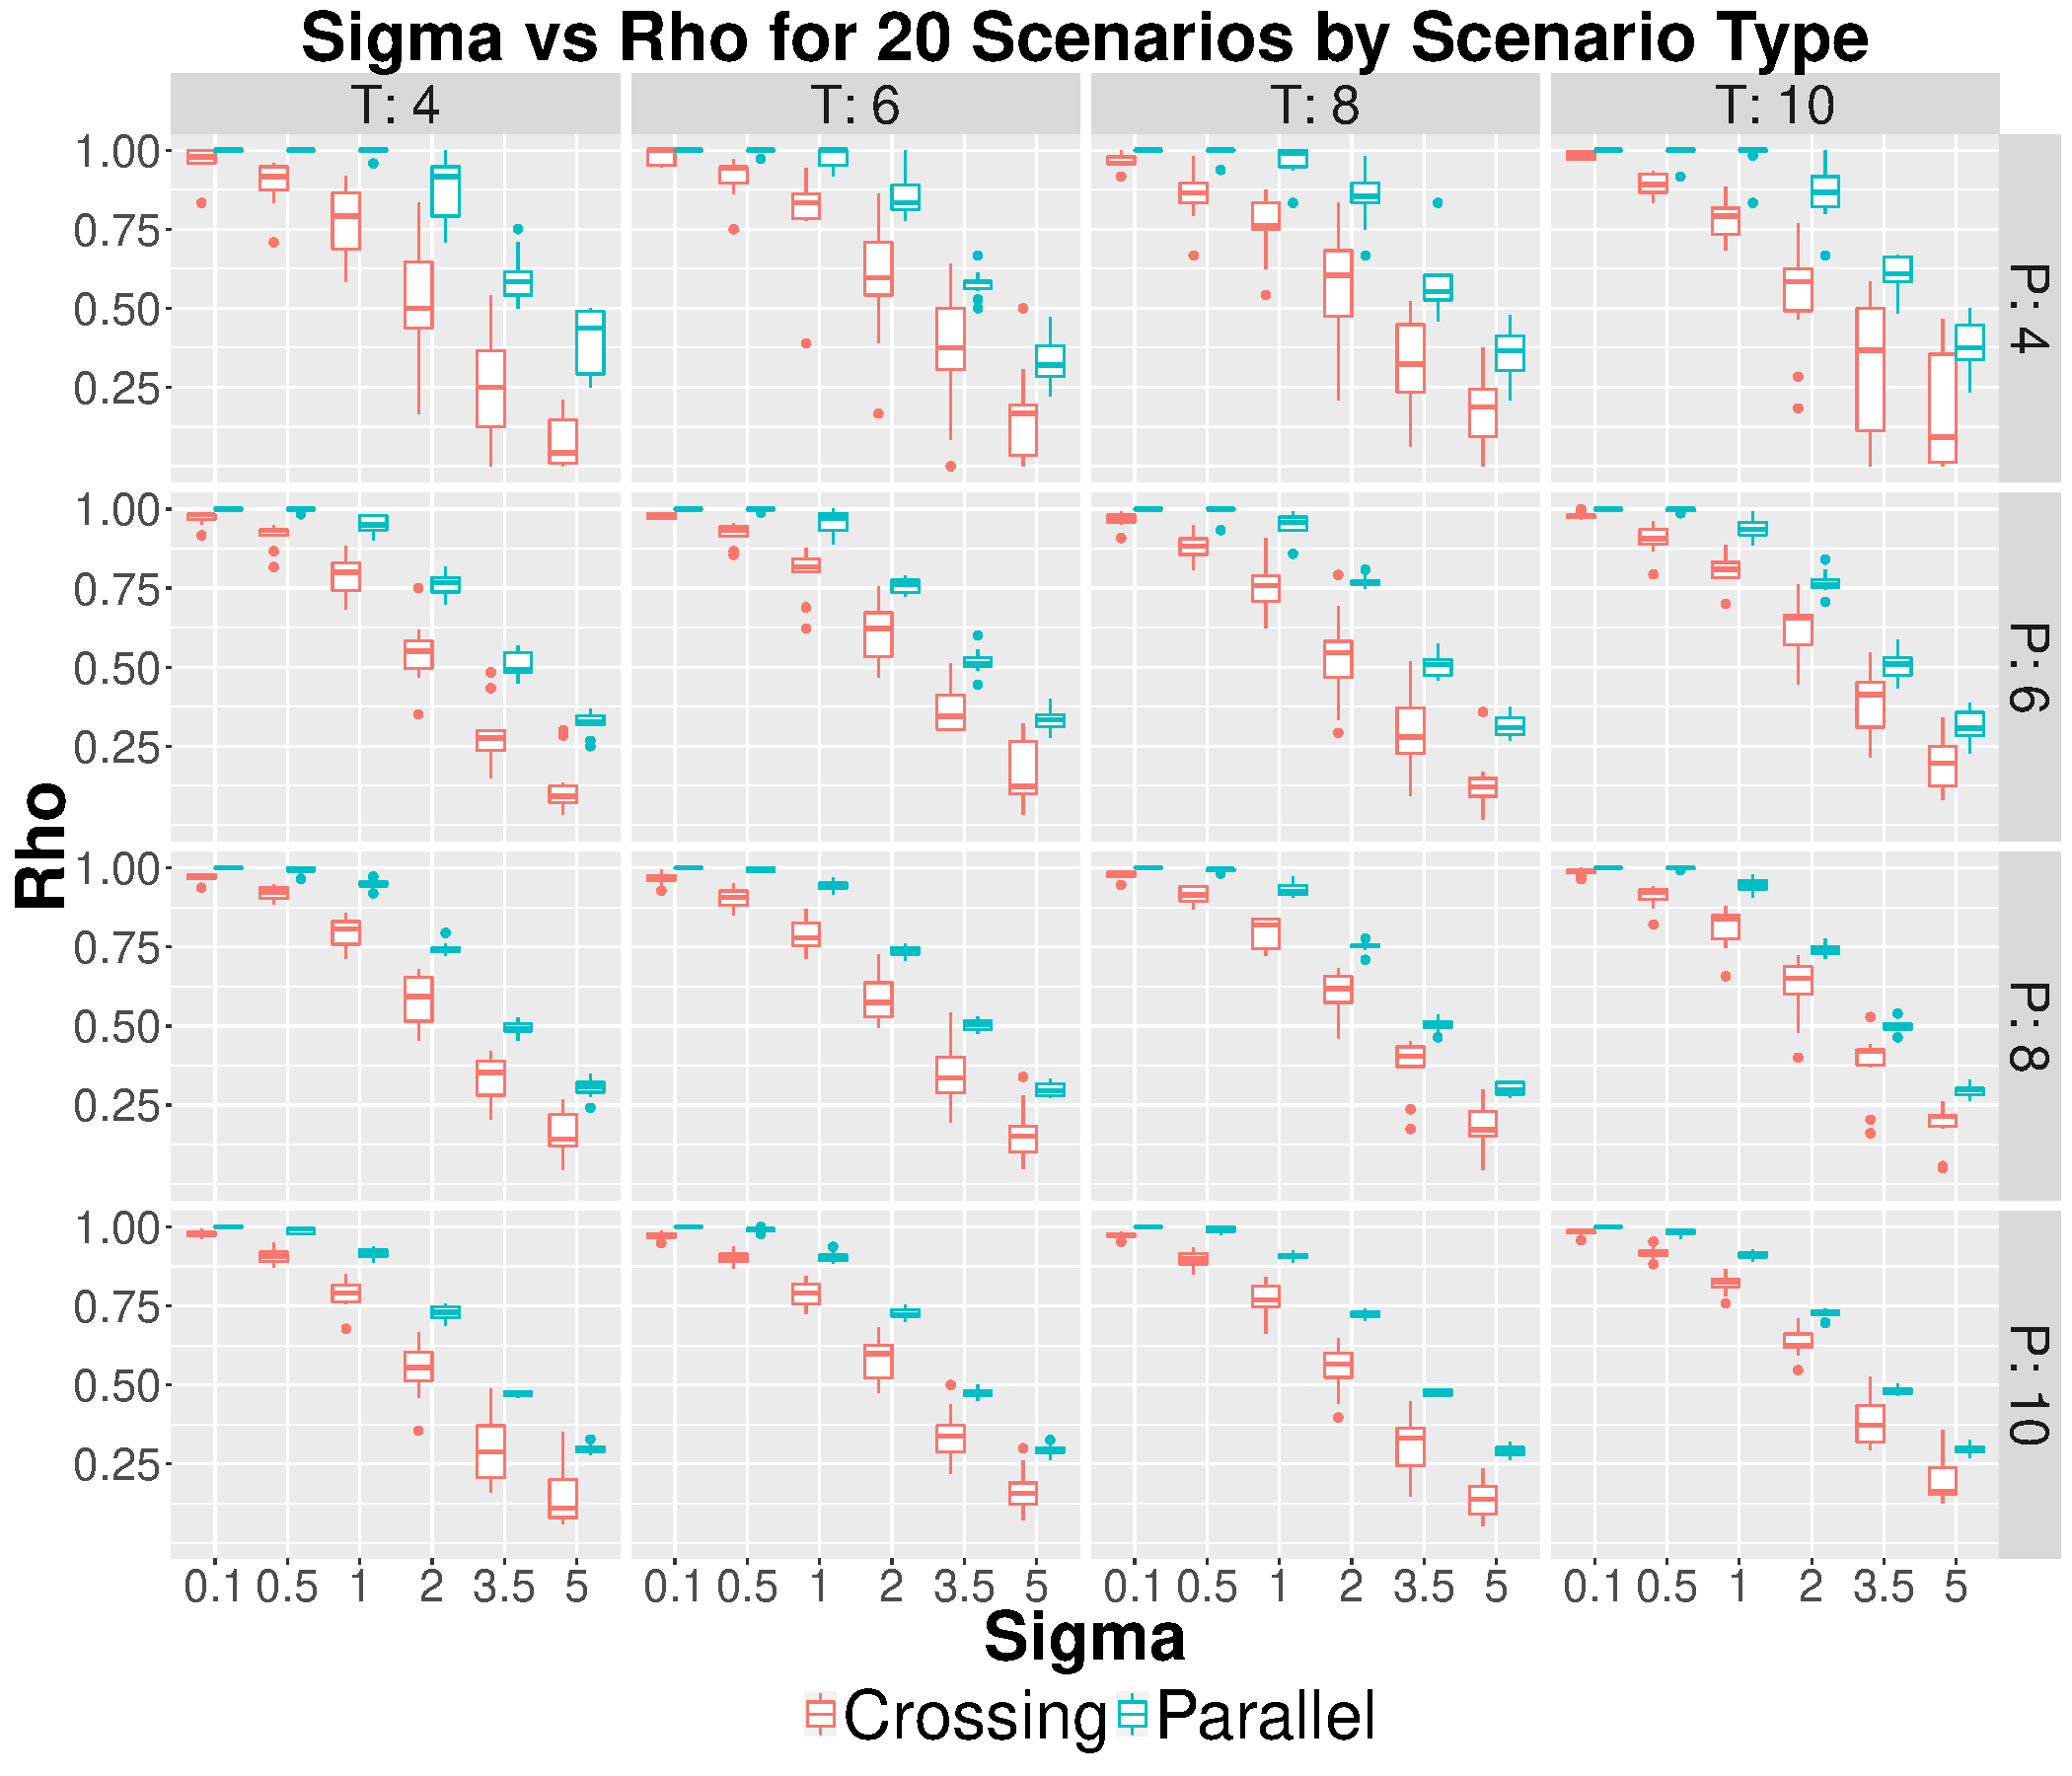
\includegraphics[width=\columnwidth]{../Figures//Sigma_vs_Rho}
    \caption{Relationship between $\sigma$ and $\rho$ summarized by scenario type for all 20 generated scenarios in this experiment.}
    \label{fig:Sigma_vs_Rho}
\end{figure}

Remember that higher values of $\rho$ indicate a {\color{red} lower} proportion of detections within very close proximity to one another. We note that the parallel method of scenario generation clearly generates easier scenarios, as measured by $\rho$. This suggests that in general, it may be more difficult to ascertain correct associations for crossing scenarios than for parallel scenarios. In addition, we can conclude from Figure~\ref{fig:Sigma_vs_Rho} that $\sigma$ and $\rho$ are {\color{red}highly correlated, and the higher $\sigma$ is the lower $\rho$ becomes, which in to be expected from the definition of $\rho$}. Furthermore, we note that {\color{red}  while $\sigma$ is restricted to a small range of six values, a wider range of possible $\rho$ values is captures, and in some instances the entire $[0,1]$ range of $\rho$ is captured. ??? why is this result beneficial? the cause and effect are not clear??? This result is beneficial to both scenario generation and complexity measuring because it suggests that $\sigma$ can be used in its natural domain of the data generation process, and $\rho$ can be back calculated as a measurement of difficulty for the data association problem.} As a result, we gain a highly interpretable performance metric for the data association problem without sacrificing the ability to generate scenarios in their natural domain.  {\color{red} Still missing - refer to a specific graph, give numerical examples of what you claim to be true}

\mysubsubsection{Basic Heuristic}
We transition to discuss performance of the heuristic, beginning with an examination of the experimental run times. Table~\ref{tab:Basic_heuristic_times} summarizes the minimum, mean, and maximum run times of the heuristic for a single starting point, arranged by the number of targets ($P$) and number of scans ($T$). Times are shown in milliseconds. 

\begin{table}[ht]
\centering
\begin{tabular}{cc|ccc}
  \hline
   & & \multicolumn{3}{c}{Heuristic Run Times } \\
   & & \multicolumn{3}{c}{(in milliseconds)}\\
   P & T & Min & Mean & Max \\ 
  \hline
  \hline
   4 & 4 & 0.07 & 0.10 & 0.18 \\ 
   4 & 6 & 0.18 & 0.24 & 0.38 \\ 
   4 & 8 & 0.34 & 0.45 & 0.62 \\ 
   4 & 10 & 0.58 & 0.76 & 1.02 \\ 
   6 & 4 & 0.11 & 0.15 & 0.25 \\ 
   6 & 6 & 0.31 & 0.39 & 0.58 \\ 
   6 & 8 & 0.64 & 0.81 & 1.05 \\ 
   6 & 10 & 1.24 & 1.56 & 2.02 \\ 
   8 & 4 & 0.14 & 0.19 & 0.30 \\ 
   8 & 6 & 0.46 & 0.57 & 0.86 \\ 
   8 & 8 & 0.95 & 1.24 & 1.58 \\ 
   8 & 10 & 2.07 & 2.53 & 3.37 \\ 
   10 & 4 & 0.19 & 0.25 & 0.41 \\ 
   10 & 6 & 0.63 & 0.80 & 1.03 \\ 
   10 & 8 & 1.44 & 1.84 & 2.44 \\ 
   10 & 10 & 2.96 & 3.73 & 4.56 \\ 
   \hline
\end{tabular}
\caption{Heuristic run times (in milliseconds) for a single starting point.}
\label{tab:Basic_heuristic_times}
\end{table}

At a glance, it is evident that the heuristic scales more efficiently with increases in the number of targets than increases in the number of scans. Notice that the average run time roughly doubles with each addition of two scans, for a fixed number of targets. {\color{red} again missing numerical examples - talk in numbers} an the other hand, the average run time never increases more than 50$\%$ for an increase of two targets, given a fixed number of scans. Therefore, we conclude that the heuristic would be capable evaluating scenarios with a surprisingly large number of targets, but measures should be taken to avoid significant increases in the number of scans. 

Implementing the heuristic as sliding window algorithm would very likely mitigate this scaling effect in regards to $T$. Rather than solve all scans in a single batch at once, a sliding window algorithm solves a subset of scans, or a smaller window, and advances through all scans sequentially.  As the window progresses forward through the scans,``soft'' decisions are made meaning that the heuristic would begin with the decisions from the previous solution. As scans pass beyond the horizon and out of the sliding window, the decisions become fixed and we refer to them as ``hard" decisions. This process continues until all scans have been processed. The run times of a sliding window variant of the heuristic would not exhibit the curse of dimensionality in $T$ since the number of scans remains constant. Additionally, the heuristic is likely to produce higher quality solutions as a result of these ``soft" decisions of previous steps since it is starting from a solution which is likely to be better than a completely random solution. 

Furthermore, the full strength of the heuristic isn't realized until we remember that the heuristic is extremely parallelizable. By running the heuristic on several processors, we can reduce the number of starting points run on each processor, reducing the total processor running time. As a result, given enough processors, the heuristic can run several thousand starting points and still find solutions in a fraction of a second. To illustrate, say that we intend to run 50,000 heuristic starting points for a scenario with six targets and six scans. The average run time for a single starting point of this size is about 0.4 milliseconds. Running all of these starting points in sequence would require approximately 20 seconds of run time, however, the same amount of starting points parallelized onto 100 processors would only require a run time on the order of 0.2 seconds. Thus, the run time of the heuristic can be reduced to meet the efficiency needs of the system subject only to the limitation of available processors. 

We have seen that the heuristic scales efficiently in regards to the number of targets, and we have also seen the power of the heuristic when parallelized, but \textit{does the heuristic provide good feasible solutions to serve as a warm start to the MIO?} In order to answer this question appropriately, we compare the heuristic solution to the ideal solution, which as a reminder is the solution in which the data association problem is exactly correct. Toward this goal we compute the MIO objective value of both the heuristic solution and the ideal solution, and report the ratio between the first value and the second. Figure~\ref{fig:Basic_Heuristic_Objective} plots this ratio against $\sigma$. {\color{red} The y axis title is misleading, I would call the MIO objective by a letter, say $f$ and compare $f_H$ vs. $f_I$ where $H$ signifies Heurtic and $I$ Ideal solutions.}
\begin{figure}[ht]
  \centering
  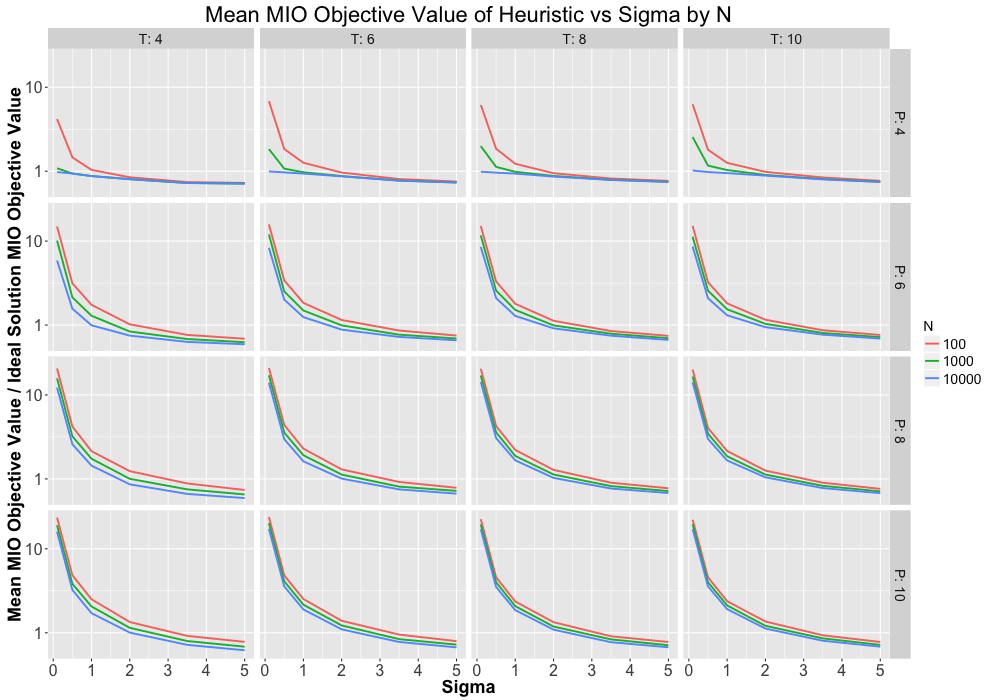
\includegraphics[width=\columnwidth]{../Figures/Basic_Heuristic_Objective}
  \caption{Quality of heuristic solution as compared to the ideal solution's MIO objective value summarized by number of starting points.}
  \label{fig:Basic_Heuristic_Objective}
\end{figure}

On the whole, we see that increasing the number of starting points improves the quality of heuristic solutions as compared to the ideal solution's MIO objective value, though the magnitude of improvement diminishes as the number of targets increases. Yet for scenarios with only four targets, we see that increasing the number of starting points has a significant effect {color{red} quantify}. This suggests that in order to maintain solution quality, the number of necessary starting points increases with $P$, likely due to the exponential increase in combinatorial solutions as the number of targets increases. Additionally, there does not appear to be a significant loss in quality as the number of scans increases, suggesting that solution quality scales efficiently with increases in $T$. Altogether, this suggests that the heuristic solution quality scales better in regards to increases in $T$ than $P$. We remind the reader that this easily mitigated due to the fact that a very large number of starting points can be evaluated efficiently through the power of parallelization. 

It is important to note that the heuristic outperforms the ideal solution's MIO objective value for larger values of $\sigma$ {\color{red} again give an example, state the outperforms = ratio smaller than 1}. Remember that the ideal solution is simply ideal in the sphere of data association, while the MIO objective function serves to quantify solutions in regards to both data association and trajectory estimation simultaneously. This result suggests that the heuristic gives a better fit to the noisy measurements but this fit does not necessarily lead to better estimated trajectories {\color{red} but we later see that in fact it does , it is simply the true association does not lead to the estimated trajectories which are closer to the true ones because of the noise}. With this in mind, we conclude that it may be necessary to tradeoff correct data associations in order to improve the trajectory estimation in cases of higher noise.

We continue our evaluation of the basic heuristic by measuring its performance on the data association problem. Figure~\ref{fig:Basic_Heuristic_Accuracy} plots the mean accuracy of each of the three quantities of starting points against $\rho$. 
\begin{figure}[ht]
  \centering
  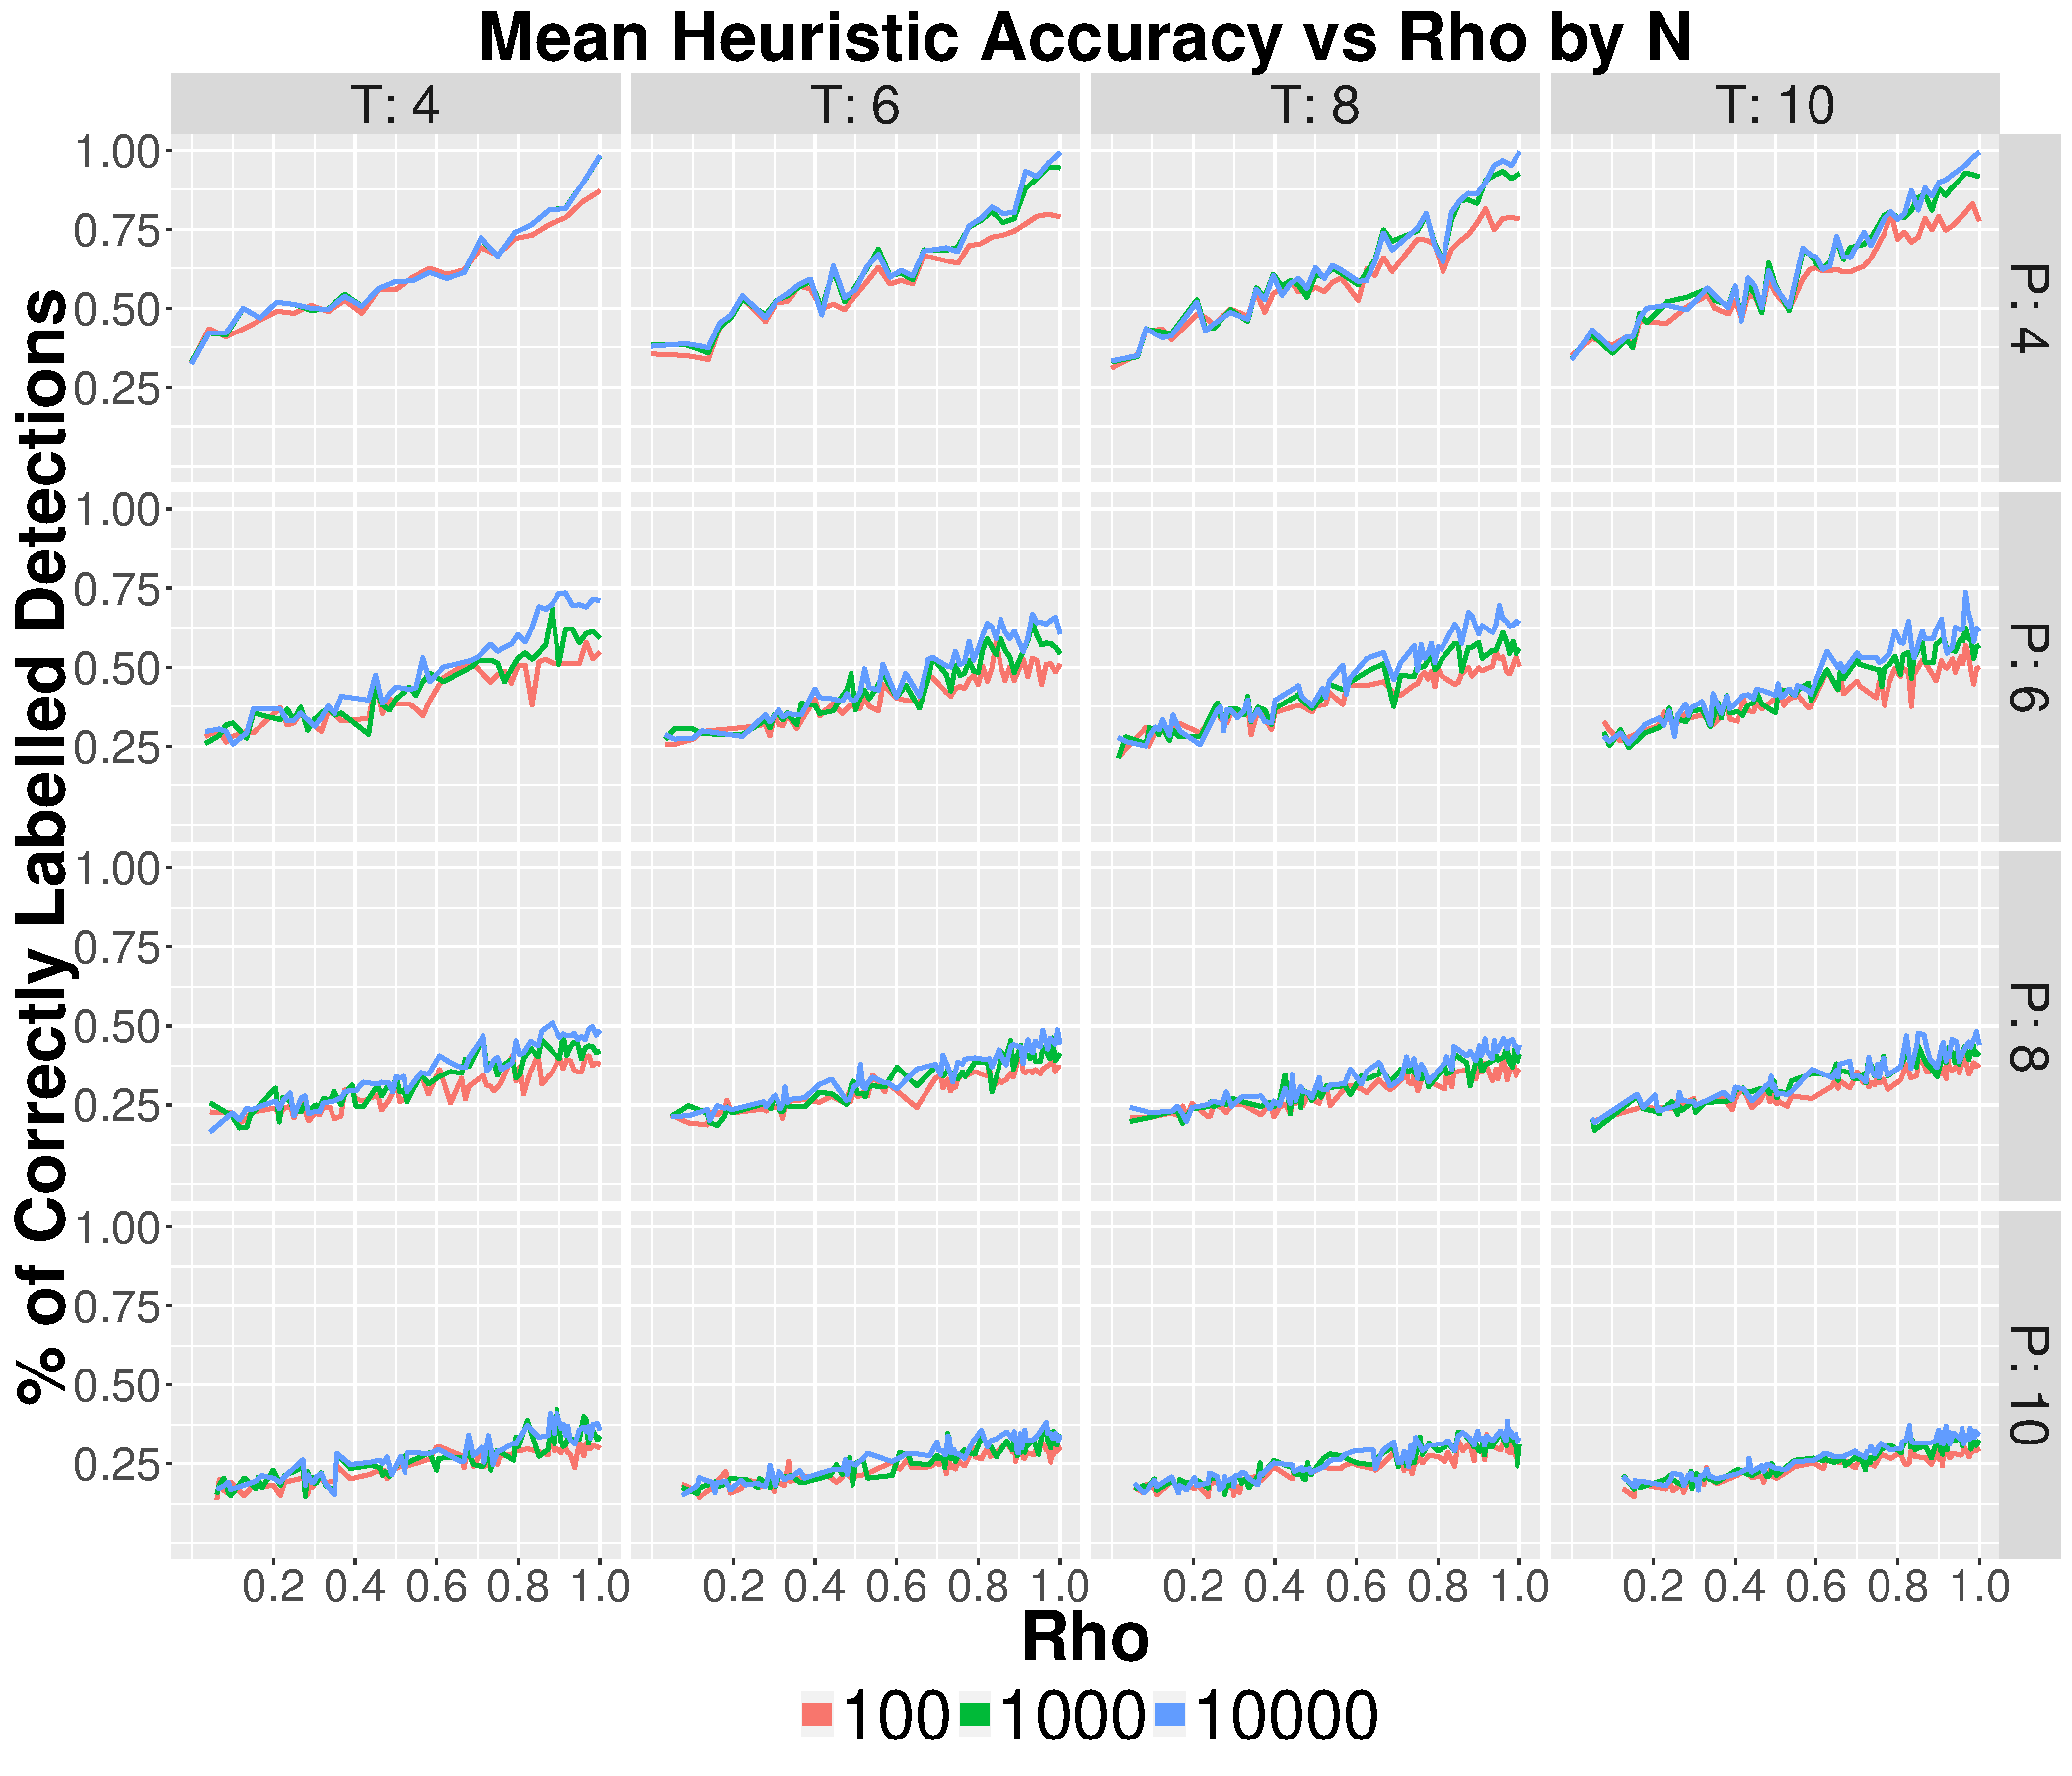
\includegraphics[width=\columnwidth]{../Figures/Basic_Heuristic_Accuracy}
  \caption{Accuracy of basic heuristic by number of heuristic starting points.}
  \label{fig:Basic_Heuristic_Accuracy}
\end{figure}

First of all, we see that the heuristic finds good solutions to the data association problem, especially {\color{red} not especially define exactly in what situations +quantify} for scenarios with fewer targets and higher values of $\rho$. While Figure~\ref{fig:Basic_Heuristic_Objective} may have instigated cause for concern of the scalability of the heuristic in regards to $P$, Figure~\ref{fig:Basic_Heuristic_Accuracy} reassures that the heuristic is adding value and finding nontrivial solutions, at least as it pertains to the data association problem {\color{red} this is not exactly true for P=10 for example, explain what you means by scale, the sentence is too general}. Perhaps this is further evidence that the ideal solution of perfect data associations does not always correspond to the best solution when balancing both data association and trajectory estimation.

Overall, we conclude that the heuristic run times scale especially well in regards to increases in the number of targets, though the solution quality may not scale quite as well. In any event, we have seen that there is not a significant difference in heuristic performance for the range of $N$ values that we explored. Therefore, for simplification as we move forward in our analysis, we will restrict our discussions of the heuristic to $N=1,000$. Next, we will see how the MIO performs. 

\mysubsubsection{Basic MIO}
We shift our focus to the MIO by first measuring its performance on the data association problem. Figure~\ref{fig:Basic_Accuracy_Summary} plots the mean accuracy of the MIO, initialized by the $N=1,000$ heuristic solutions, after 1,T, and 2T seconds against $\rho$. Note that we excluded the data for the MIO after 3T seconds for the sake of clarity as it showed little to no improvement over the MIO solution after 2T seconds. Also note that the ideal solution, which always achieves an accuracy of 1.0, has also been excluded. For comparison, we have included the accuracy of random solutions. 
\begin{figure}[ht]
  \centering  
  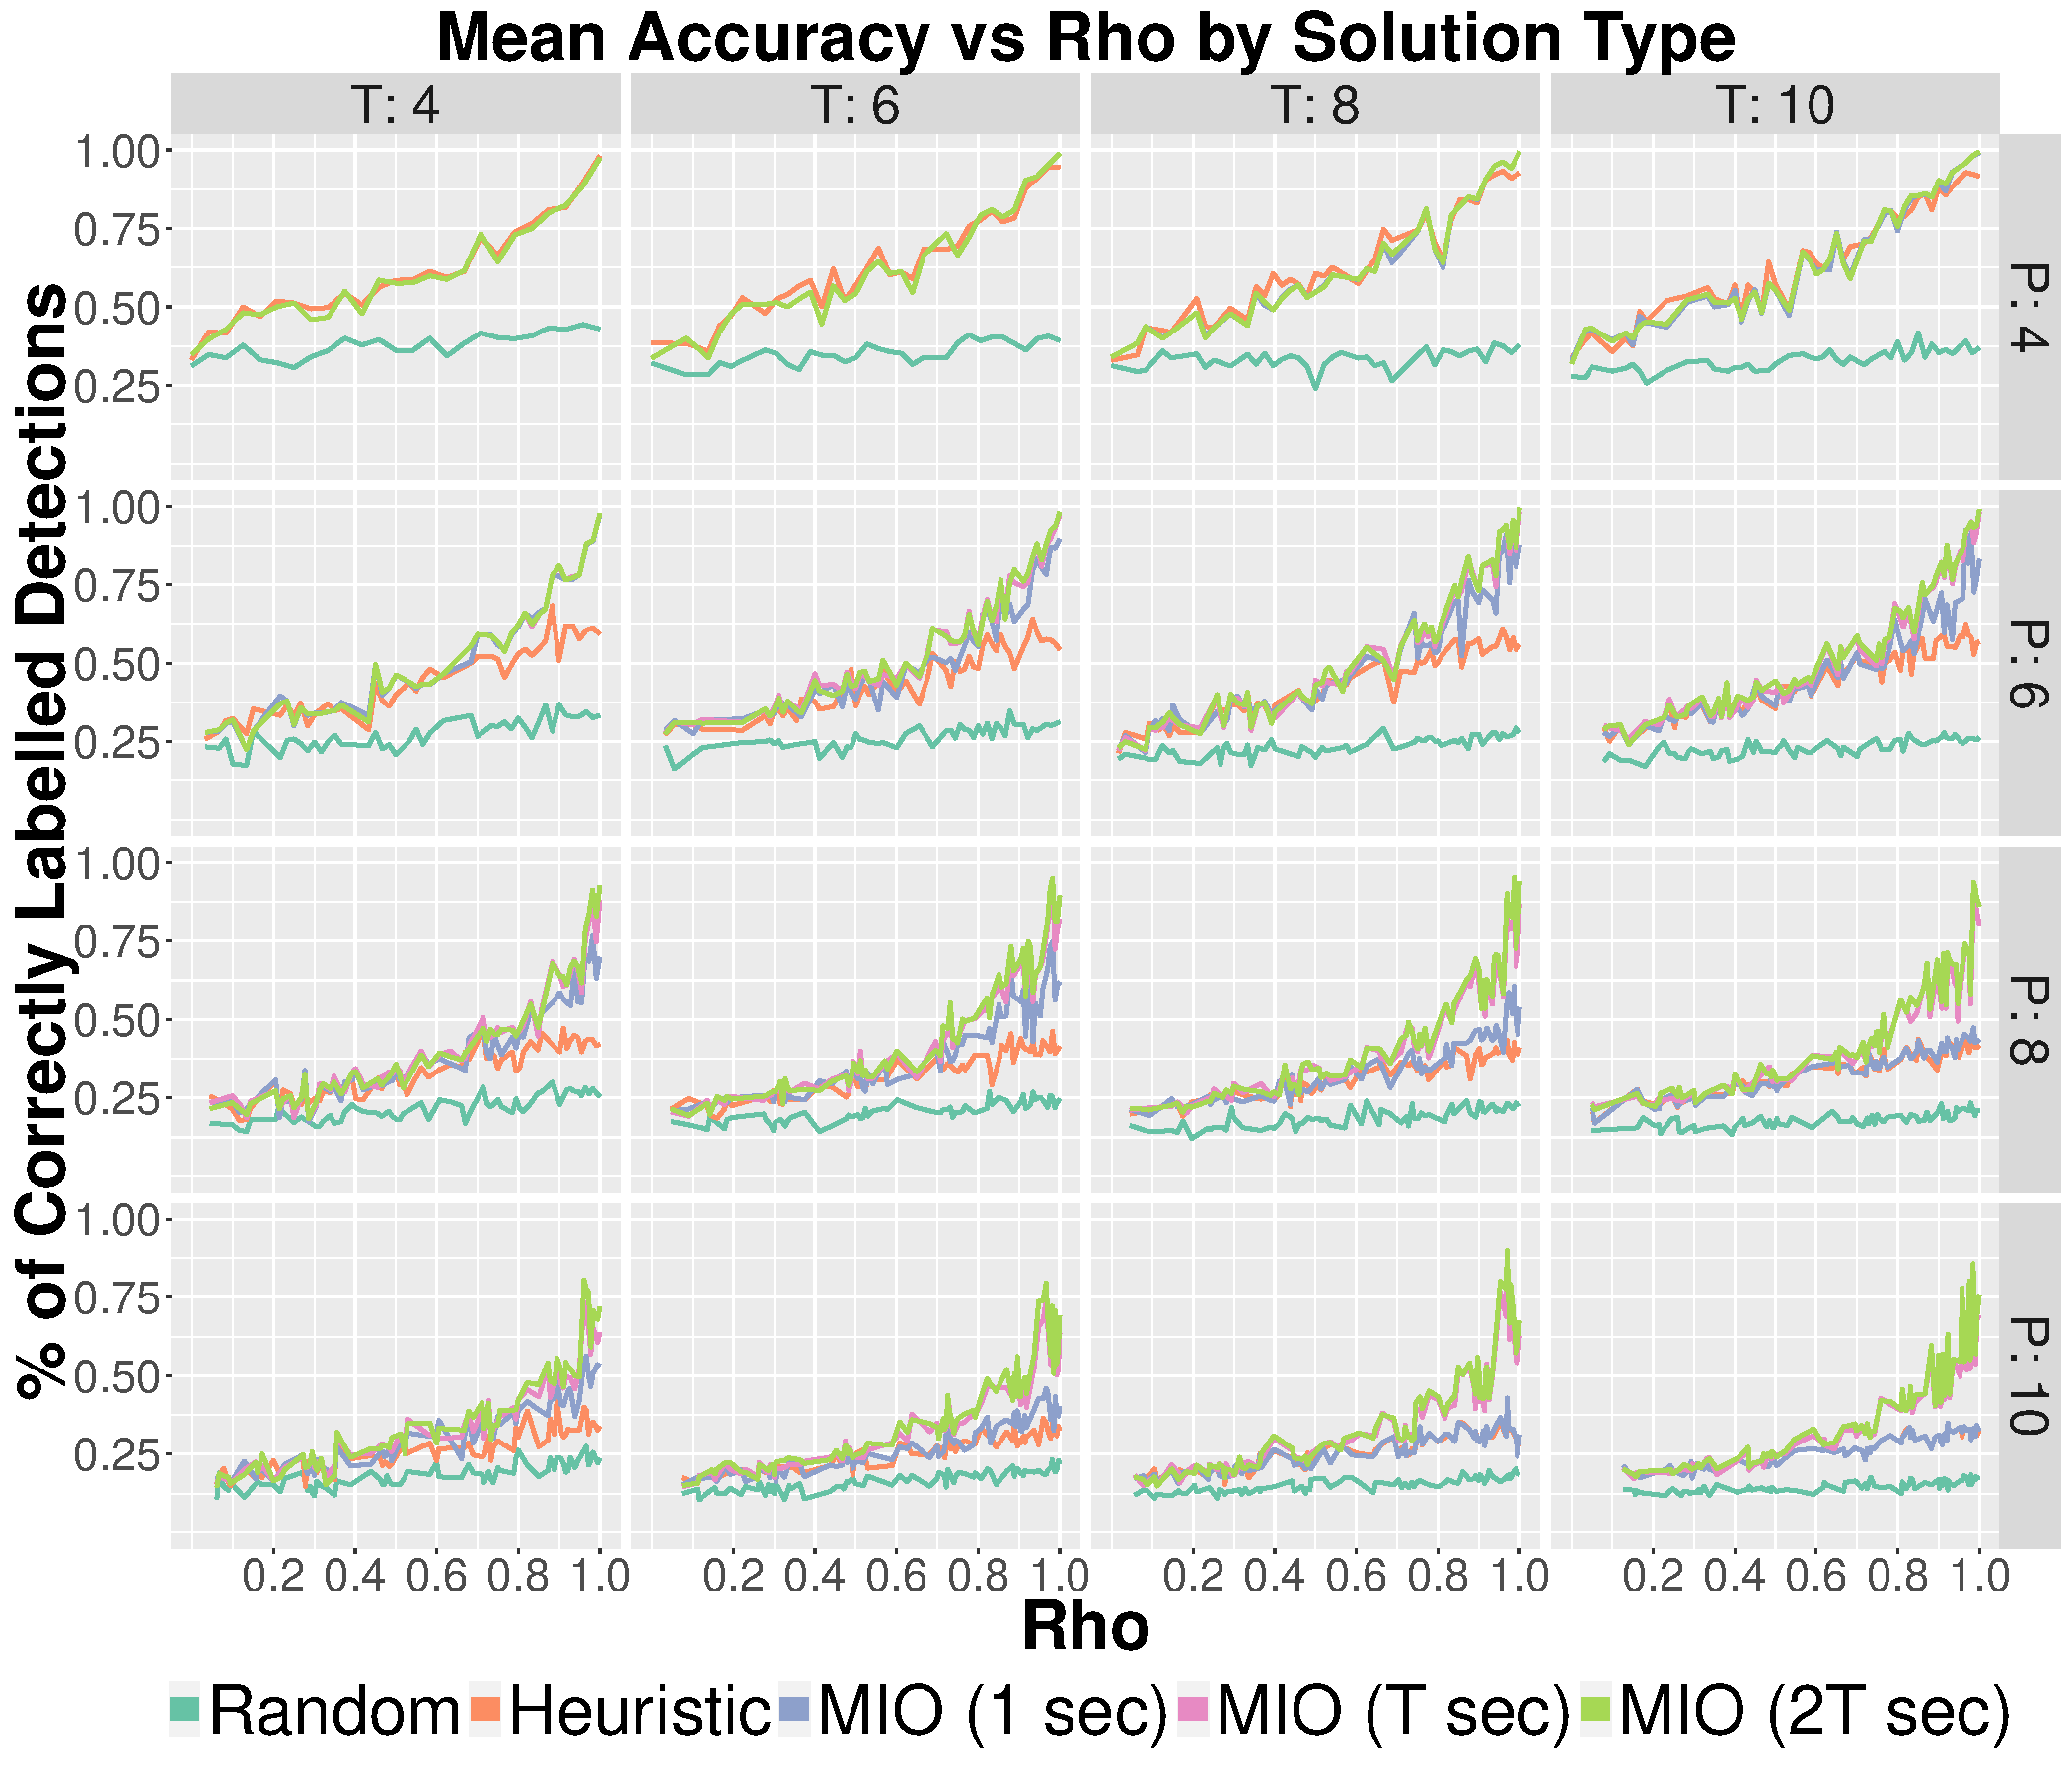
\includegraphics[width=\columnwidth]{../Figures/Basic_Accuracy_Summary}
  \caption{Accuracy of MIO compared against the heuristic and a randomized solution.}
  \label{fig:Basic_Accuracy_Summary}
\end{figure}

The MIO finds high quality solutions to the data association problem, and it appears to scale fairly well in regards to increases in both $P$ and $T$. For all scenarios with eight or fewer targets, accuracy tops out at or near {\color{red} "near" not a good word, quantify, in which cases?} in 1.0, and reduces to about 0.85 for ten target scenarios. Furthermore, scenarios with ten scans appear to slightly outperform scenarios with only four scans, suggesting that additional scans benefit the MIO solution quality, likely due to the added information gathered from an increase in the number of detections. 

While not seen in Figure~\ref{fig:Basic_Accuracy_Summary}, we note that for scenarios with four targets, many of the MIO solutions were actually proven to be the optimal solution. The fact that the heuristic performance is almost identical to the MIO again suggests that the heuristic finds high quality solutions. This is further supported by the fact the heuristic performs almost as well as the MIO after 1 second even in scenarios with ten targets. Equally as important, Figure~\ref{fig:Basic_Accuracy_Summary} shows that in nearly all scenarios, the MIO achieves its best or near best solutions after $T$ or fewer seconds, suggesting the usefulness of the MIO as an online algorithm with a sliding window. As mentioned previously in regards to the heuristic,{\color{red} why are you repeating the same thing? maybe condense or just talk about the MIO implementation in this case} a sliding window algorithm would make decisions on a subset of scans, and these decisions will be fixed before accepting a new set of scans. In regards to the MIO, this would be implemented by adding constraints to restrict the values of $y_{itj}$ to match that of the subsetted solution. The fact that the MIO finds very good solutions in $T$ or fewer seconds means that a sliding window algorithm would be able to solve each subset in real time before advancing to the next subset of scans. Furthermore, the MIO would likely benefit from the fixed decisions of the preceding windows, since {\color{red} the fact we have not utilized it does not explain why it will benefit the MIO and what is "our approaches"} this is added knowledge that has not utilized by our approaches.

Next, we evaluate the performance of the basic heuristic and MIO through the lens of trajectory estimation. As discussed previously, we are interested in comparing $\delta$, our proxy for ground track error, against $\sigma$, our measure of difficulty for trajectory estimation, in order to analyze performance of in the sphere of estimation. Figure~\ref{Fig:Basic_Delta_Summary} plots $\sigma$ against $\delta$ for each of the solution types. In addition to the random solution shown on the previous plot, we also add a comparison to the ideal solution, which was previously defined.
\begin{figure}[ht]
  \centering
  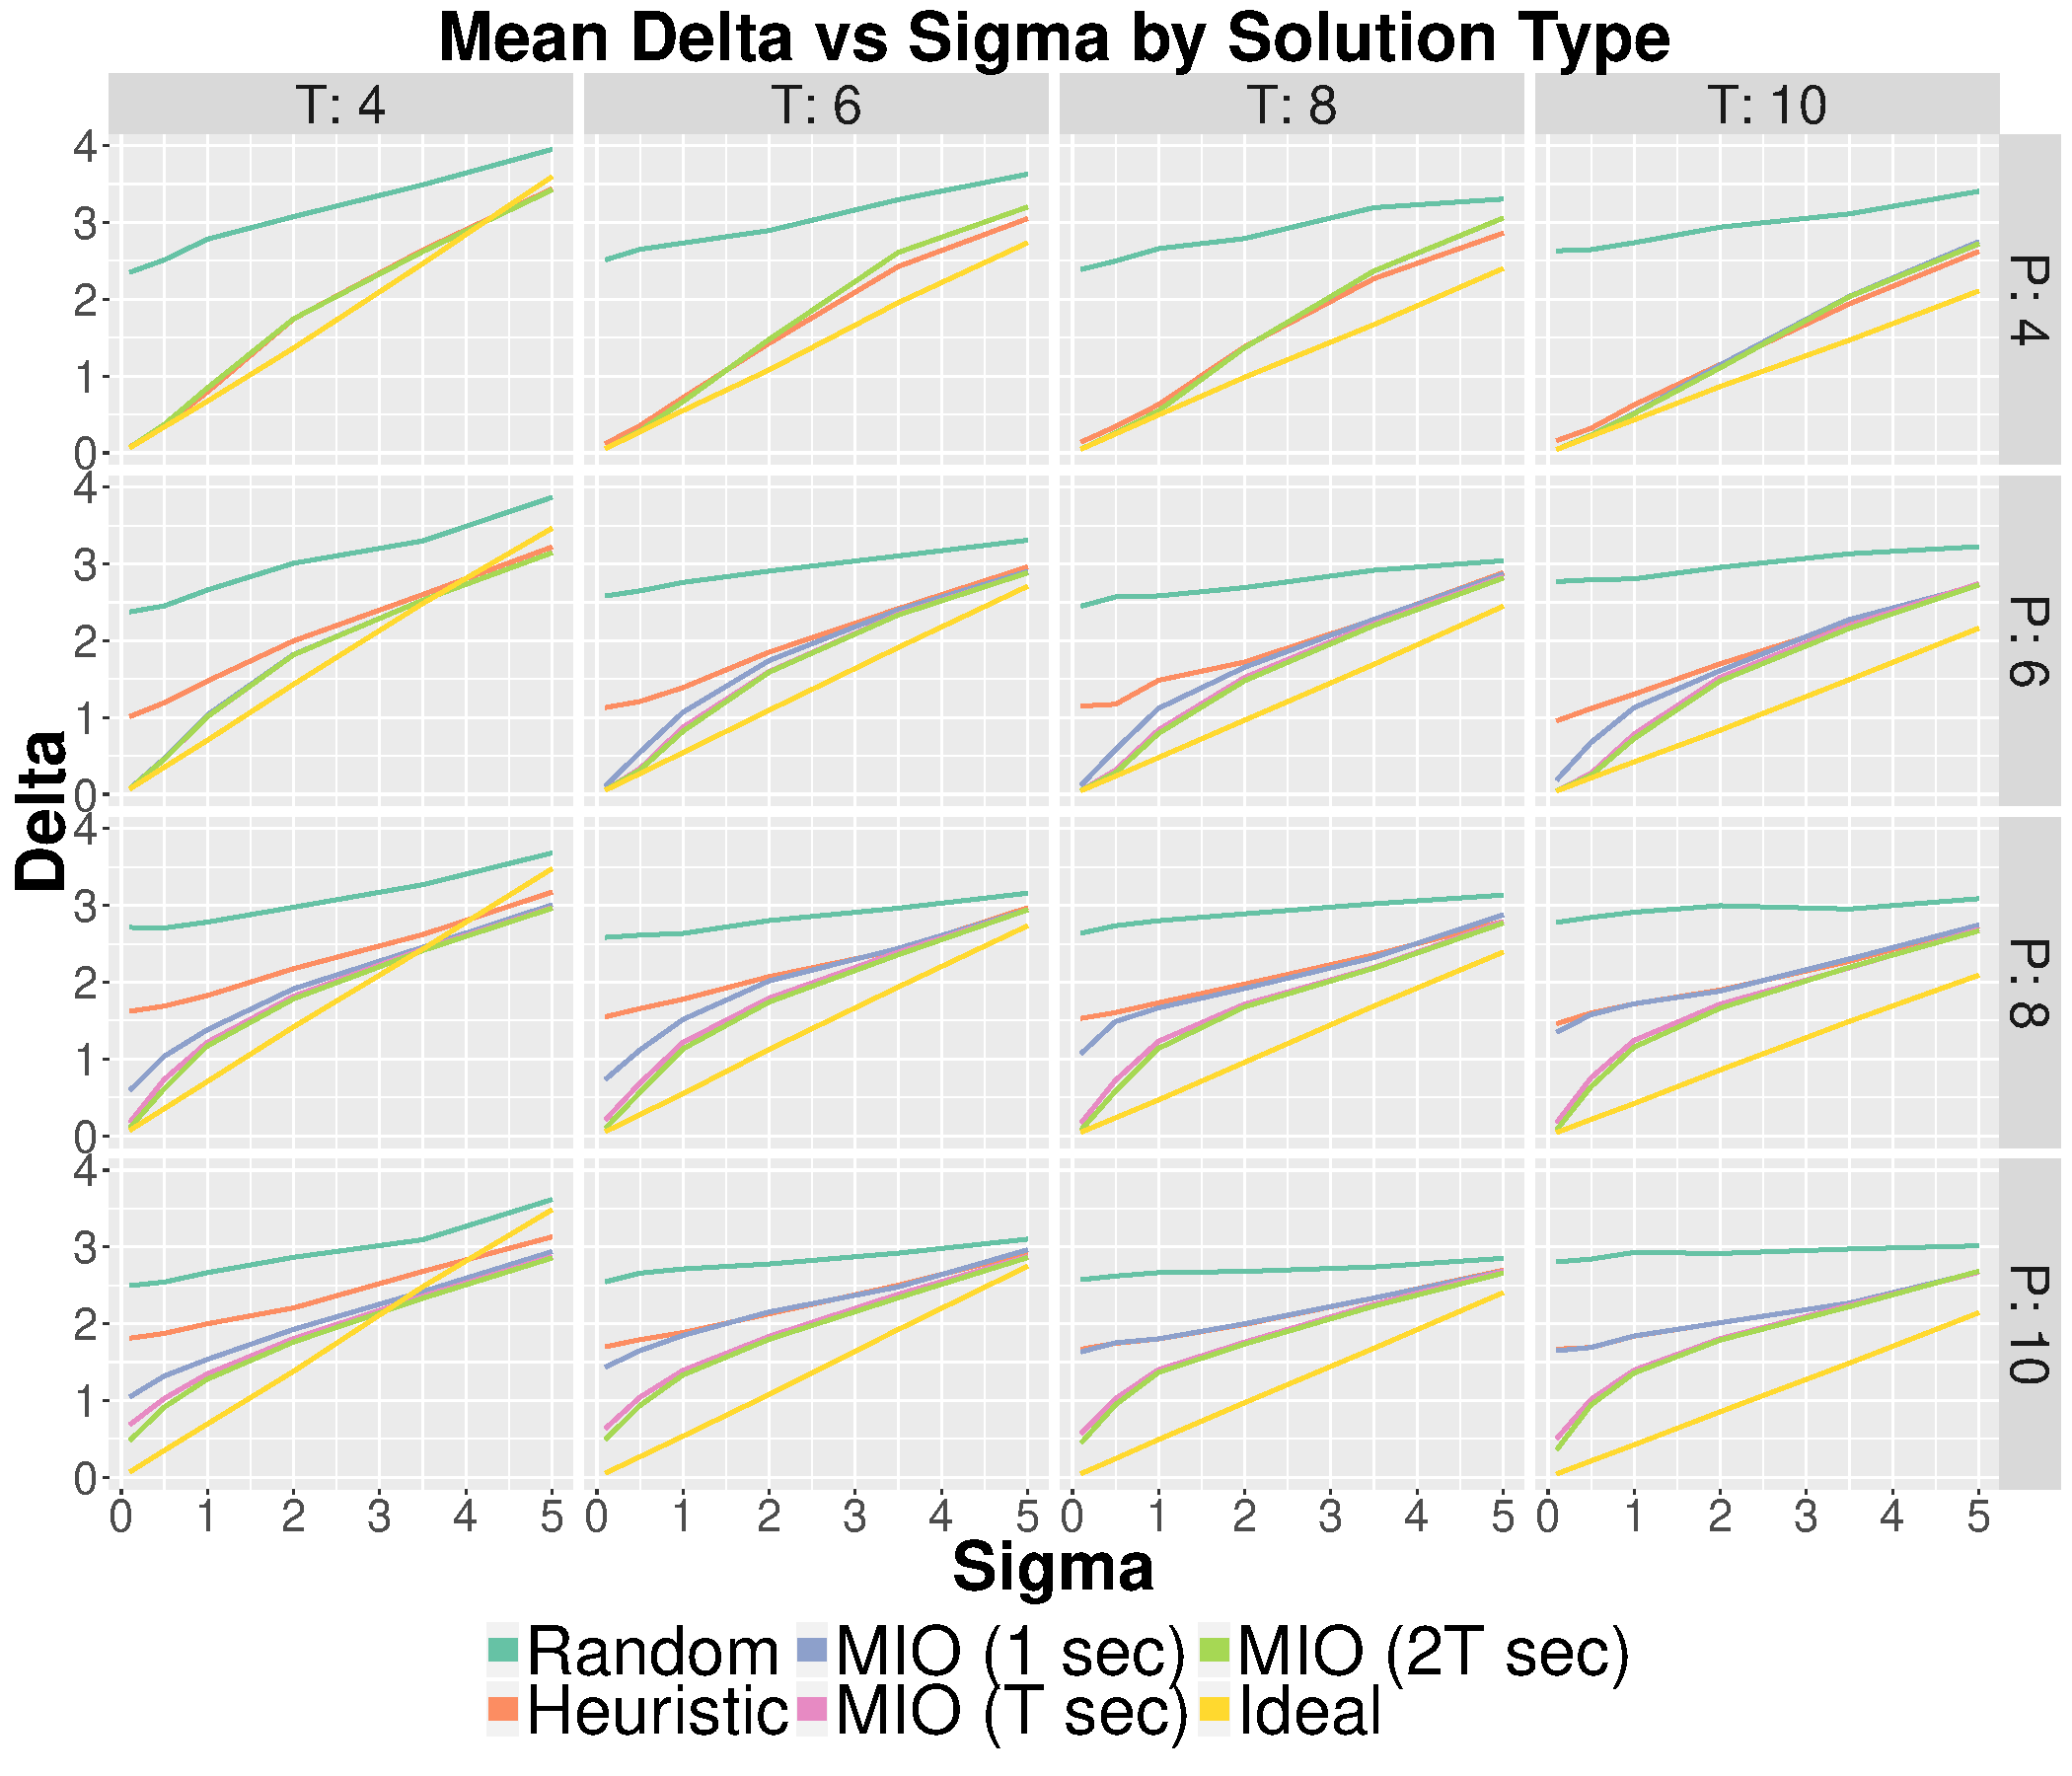
\includegraphics[width=\columnwidth]{../Figures/Basic_Delta_Summary}
  \caption{Trajectory estimation performance}
  \label{Fig:Basic_Delta_Summary}
\end{figure}

Remember that lower values of delta correspond to trajectory estimations that are closer to that of the true ground track. We see that the performance of the heuristic converges to that of the MIO for scenarios with few targets, as well as for large values of $\sigma$ {\color{red} quantify}. Additionally, we see that as the number of targets increases we begin to see stronger improvements by the MIO over the heuristic. Interestingly, we see that for the scenarios with the largest number of targets and scans, the MIO after one second is not much better than the heuristic, while the MIO after T seconds provides significant improvement over that of the heuristic and MIO after 1 second, there is little further improvement in running the MIO for 2T seconds. {\color{red} explain why this happens, why only for large number of targets} 

Again, we see that \sout{occasionally} the heuristic and/or MIO outperform(s) the ideal solution \sout{especially for} in scenarios with only four scans {\color{red} and high values of $\sigma$}. This effect increases as the value of $\sigma$ increases. This result suggests that as the number of scans approaches infinity, the estimated trajectories given by the ideal association approaches the true ground tracks. Put differently, as more and more data is available, it becomes easier to estimate the trajectories even in the event of \sout{large} low signal to noise ratio, and so the trajectory estimates that result from the ideal solution converges to the true ground track. {\color{red} but what does this have to do with the MIO? and the phenomenon you just described?}

In summary, we have shown that in the case of no detection ambiguity, the heuristic is scalable, particularly in regards to increases in the number of targets, and it finds high quality solutions in milliseconds. The MIO is also scalable, appearing relatively robust to both increases in the amount of targets and scans. Both approaches show promising signs for use in a sliding window algorithm.

\mysubsection{Scenarios with Detection Ambiguity}
Here we extend the discussion from the previous section to analyze the performance of our methods on scenarios with detection ambiguity. We first summarize our experimental methods before discussing performance of both the robust heuristic and the robust MIO in the spheres of both the data association and trajectory estimation problems.

This experiment serves as an extension of the basic one, in order to test the performance of our algorithms under detection ambiguity. We use the same scenarios generated from the basic experiment, but due to the additional difficulty inherent with detection ambiguity, we limit the range of signal noise to $\sigma \in \{0.1,0.5,1.0,2.0\}$, excluding choosing to exclude the extreme cases of signal noise. In addition, we simulate both missed detections and false alarms. A detection is removed with probability, $\gamma$, and we consider $\gamma \in \{0.2,0.15,0.1,0.05\}$. We do not allow empty scans. For each scan, we generate false alarms according to a poisson distribution with parameter, $\lambda$, and detection locations are then randomly selected uniformly within the state space. We consider $\lambda \in \{0.1,0.5,0.1,2.0\}$. The false alarms are then added to $\mathcal{X}_{t}$ and the detection order of $\mathcal{X}_{t}$ is again randomly shuffled as before. 

Once the data has been generated, we follow the same sequence as before in the basic experiment, running the heuristic first and then feeding the solution into the MIO as a warm start. Note that the heuristic is given 1,000 starting points only, as concluded from the results of the basic experiment. Once again, the optimization process was set to terminate after 3T seconds, with solutions collected at intervals of $\{1,T,2T,3T\}$ seconds. Prior to the running of this experiment, we performed a mini experiment and used the results to tune the penalties $\theta$ and $\phi$. A summary of the exact penalties used along with an explanation of the insight behind them, can be found in Appendix~\ref{app:Penalty_Appendix}. 

We will now evaluate the performance of the robust heuristic and MIO. We begin with a discussion on the run times of the robust heuristic, following the number of targets estimation, accuracy and trajectory estimation.

\mysubsubsection{Robust Heuristic Run Times} Table~\ref{tab:Robust_heuristic_times} summarizes the minimum, mean, and maximum run times of the heuristic from Experiment 2 for a single starting point, arranged by the number of estimate targets ($P_{estimated}$) and number of scans ($T$). Times are shown in milliseconds. 

\begin{table}[ht]
\centering
\begin{tabular}{cc|ccc}
  \hline
   & & \multicolumn{3}{c}{Heuristic Run Times } \\
   & & \multicolumn{3}{c}{(in milliseconds)}\\
   $ P_{\text{estimated}}$ & T & Min & Mean & Max \\ 
  \hline
  \hline
  2 & 4 & 0.15 & 0.23 & 0.41 \\ 
  2 & 6 & 0.42 & 0.56 & 0.93 \\ 
  2 & 8 & 0.77 & 1.04 & 2.24 \\ 
  2 & 10 & 1.27 & 1.73 & 20.23 \\ 
  4 & 4 & 0.15 & 0.34 & 1.04 \\ 
  4 & 6 & 0.50 & 0.94 & 2.69 \\ 
  4 & 8 & 1.09 & 1.88 & 3.87 \\ 
  4 & 10 & 2.12 & 3.25 & 13.51 \\ 
  6 & 4 & 0.14 & 0.42 & 0.96 \\ 
  6 & 6 & 0.57 & 1.29 & 4.45 \\ 
  6 & 8 & 1.33 & 2.66 & 75.28 \\ 
  6 & 10 & 2.53 & 4.61 & 18.69 \\ 
  8 & 4 & 0.16 & 0.50 & 1.10 \\ 
  8 & 6 & 0.60 & 1.59 & 3.46 \\ 
  8 & 8 & 1.38 & 3.37 & 6.87 \\ 
  8 & 10 & 2.63 & 5.84 & 12.40 \\ 
  10 & 4 & 0.18 & 0.55 & 1.10 \\ 
  10 & 6 & 0.72 & 1.82 & 3.98 \\ 
  10 & 8 & 1.53 & 3.96 & 8.18 \\ 
  10 & 10 & 3.42 & 6.93 & 13.93 \\ 
  12 & 4 & 0.16 & 0.56 & 0.99 \\ 
  12 & 6 & 0.99 & 1.95 & 3.96 \\ 
  12 & 8 & 1.74 & 4.33 & 8.69 \\ 
  12 & 10 & 3.40 & 7.71 & 15.10 \\ 
   \hline
\end{tabular}
\caption{Robust heuristic run times (in milliseconds) for a single starting point.}
\label{tab:Robust_heuristic_times}
\end{table}

Comparing Table~\ref{tab:Basic_heuristic_times} and Table~\ref{tab:Robust_heuristic_times} we see that the run times for an estimated number of targets in the robust heuristic range from roughly double to three and four times that of a comparable number of targets in the basic heuristic. Due to the increase in combinatorial solutions in the robust heuristic over the basic heuristic, this was an expected result. The robust heuristic, however, can be parallelized in the same many as the basic heuristic, meaning that the robust heuristic can actually recover the speed of the basic heuristic with the introduction of additional processors. More importantly, we see that the robust heuristic scales very efficiently with $P_{\text{estimated}}$, and this the scaling actually improves as the number of estimated targets and scans increases. Increasing from two to six estimated targets for four scans roughly triples the run time, while increasing from eight to twelve estimated targets for four scans increases the run time by only 12\%. This is a great result because it means that a relatively wide range of estimated targets can be parallelized without fear of one subset requiring a substantially longer run time than another. 

Although the robust heuristic scales well with the number of estimated targets, it is more sensitive to increases in the number of scans. However, this effect is no worse than what we saw for the basic heuristic. It appears that on average increasing the number of scans by 2 results in a doubling of the run time for a fixed number of estimated targets. We conclude that these results again support the use of the robust heuristic in an online algorithm with a sliding window, as discussed in the previous section.
 
\mysubsubsection{Evaluating the Number of Targets}
Next, we continue our analysis of the robust approaches by quantifying the algorithms' ability to estimate the correct number of targets. This is perhaps the most important goal of a MTT algorithm and so we begin our analysis here. To this end, we define
\begin{align}
	P_{\text{diff}} = P_{\text{true}} - P_{\text{est}}
\end{align}

where $P_{\text{estimated}}$ is the number of estimated targets and $ P_{\text{true}}$ is the number of true targets, and we plot the distribution of $P_{\text{estimated}}$. Figure~\ref{fig:Robust_4_8_Histogram} shows the distribution of $P_{\text{difference}}$ for scenarios with four targets and eight scans, and for comparison, Figure~\ref{fig:Robust_8_8_Histogram} plots the same result for scenarios of eight targets and eight time scans. 
\begin{figure}[ht]
  \centering
  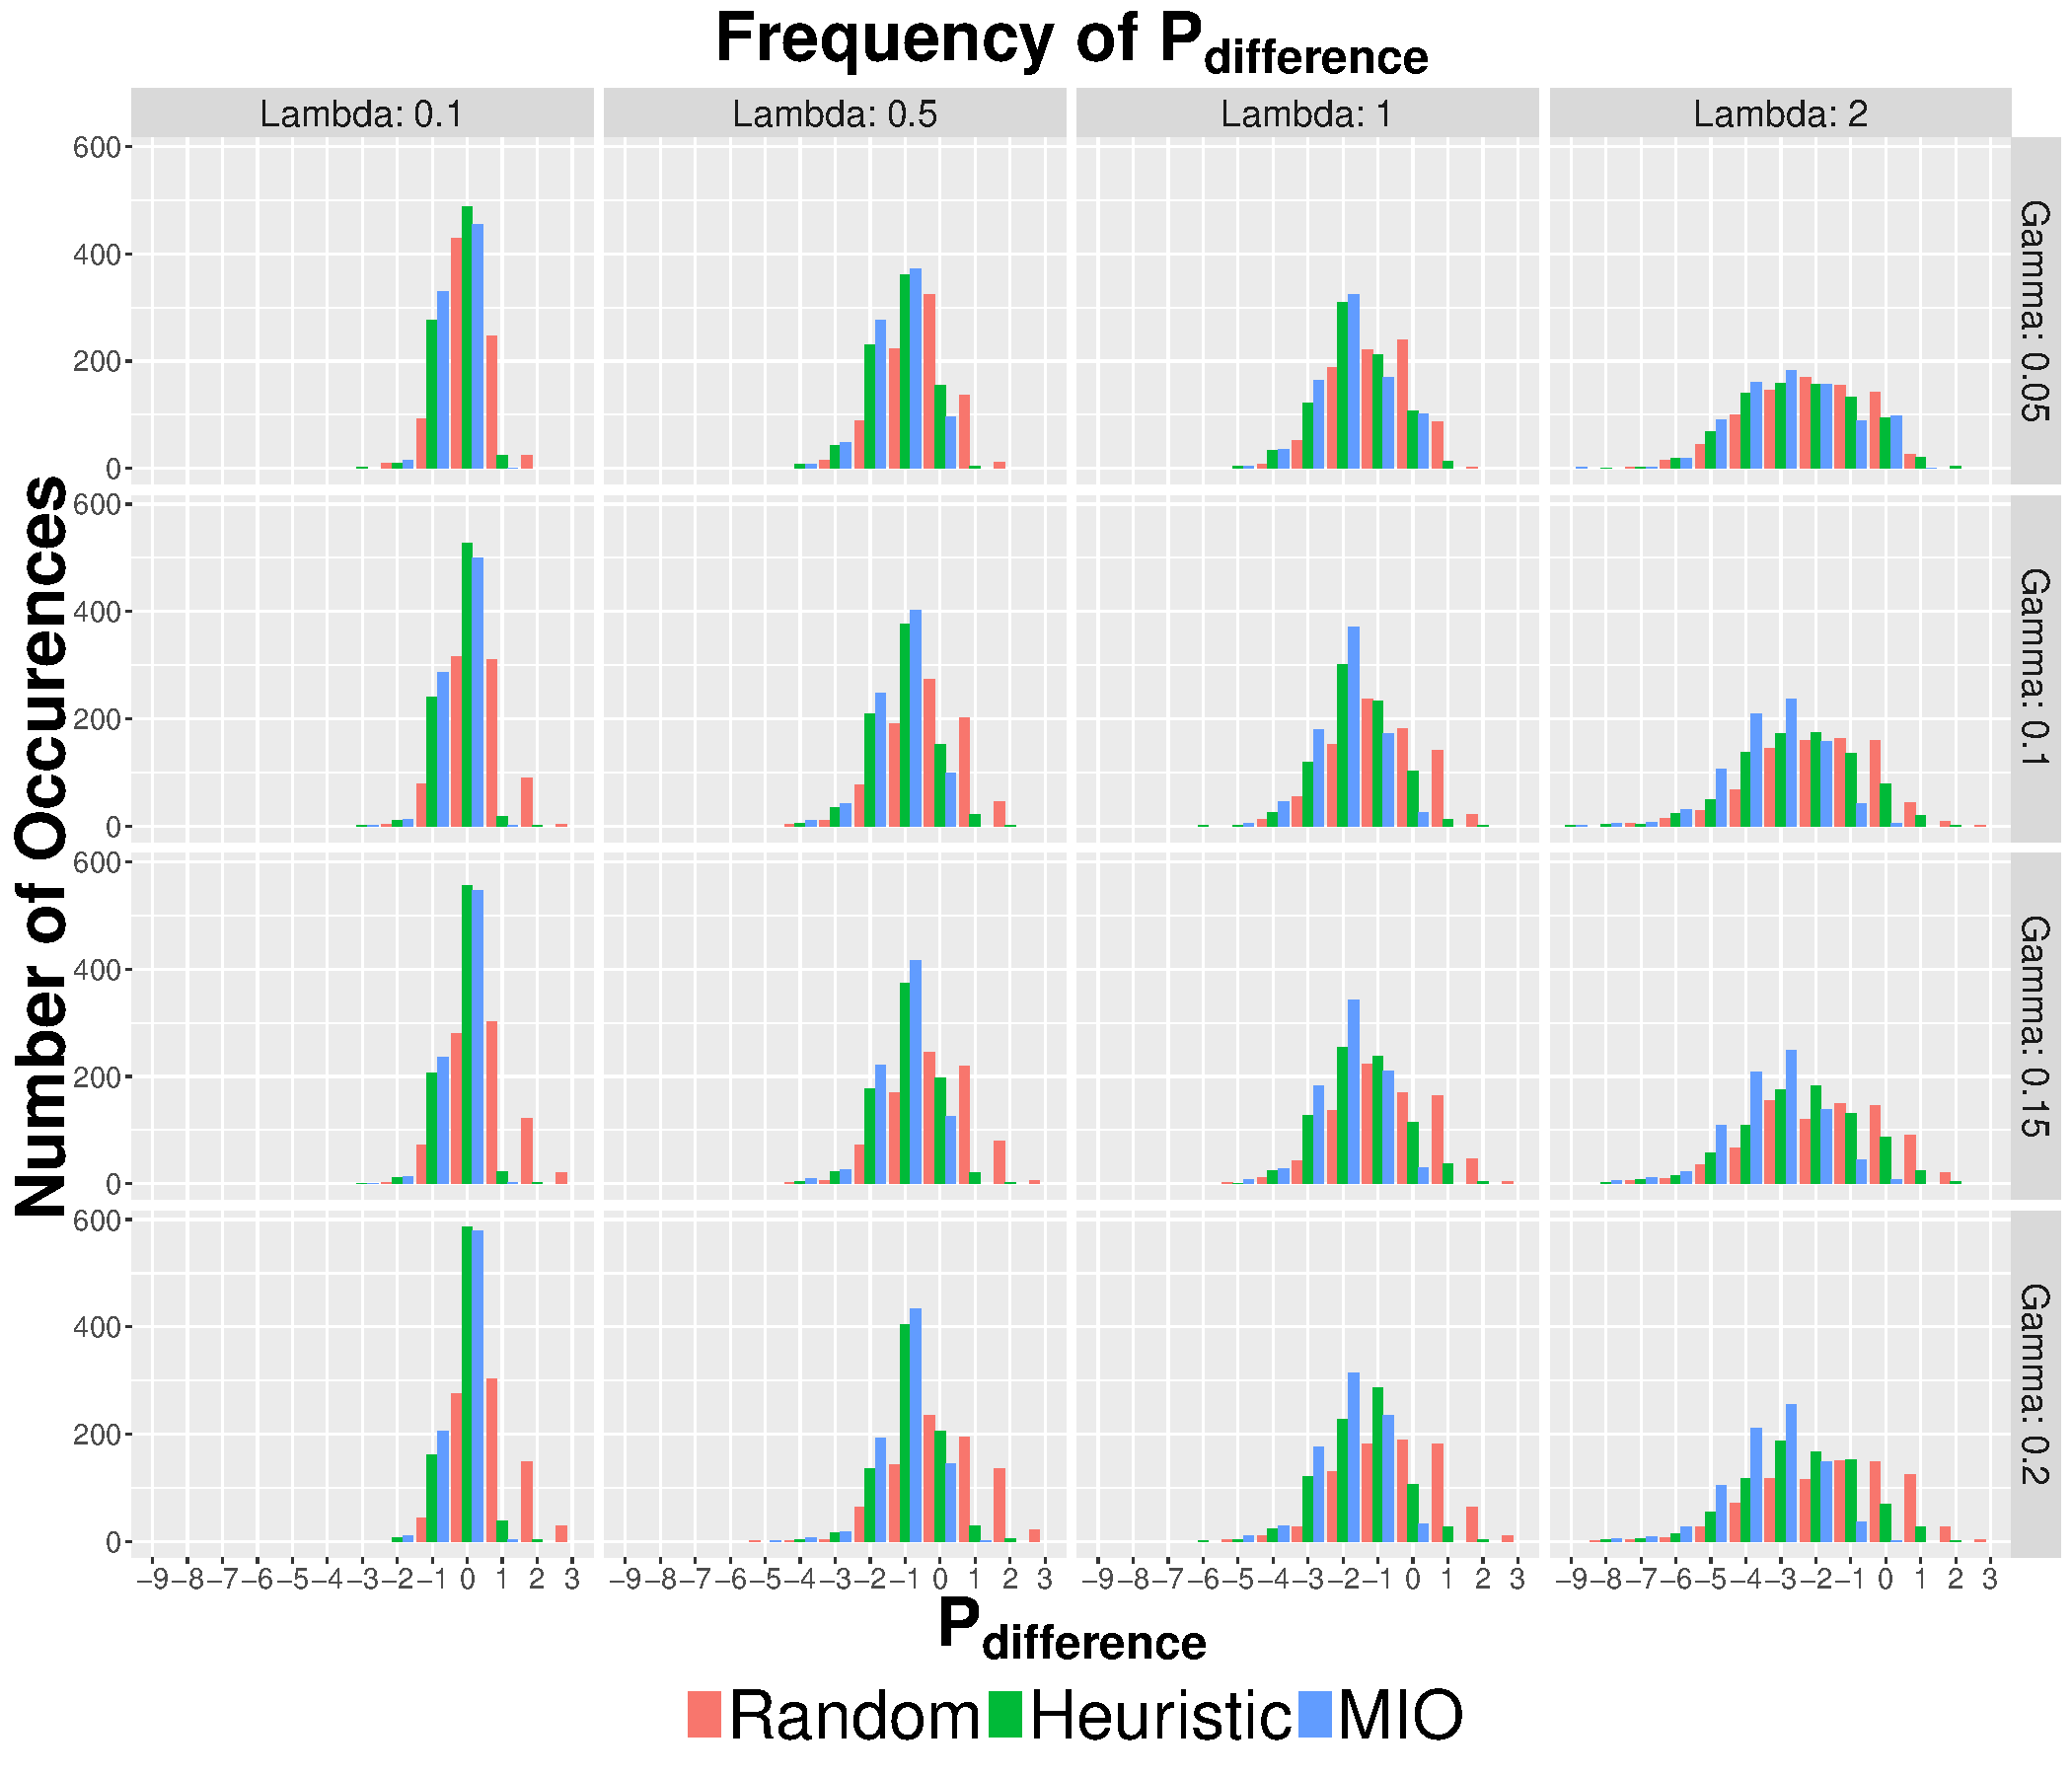
\includegraphics[width=\columnwidth]{../Figures/4_8_Histogram}
  \caption{Distribution of the difference in true and estimated number of targets for scenarios with 4 targets and 8 scans, arranged by $\gamma$ and $\lambda$.}
  \label{fig:Robust_4_8_Histogram}
\end{figure}

\begin{figure}[ht]
  \centering
  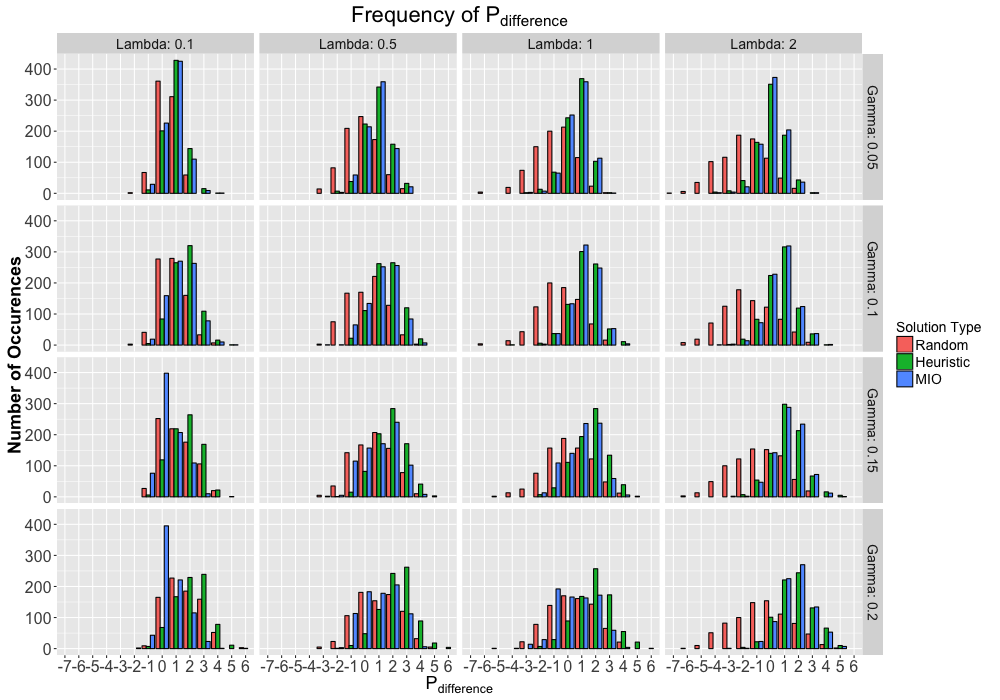
\includegraphics[width=\columnwidth]{../Figures/8_8_Histogram}
  \caption{Distribution of the difference in true and estimated number of targets for scenarios with 8 targets and 8 scans, arranged by $\gamma$ and $\lambda$.}
  \label{fig:Robust_8_8_Histogram}
\end{figure}

Note that the algorithms have correctly estimated the number of targets when $P_{\text{difference}} = 0$. When $P_{\text{difference}} < 0$, we have overestimated the number of targets, and when $P_{\text{difference}} > 0$, we have underestimated the number of targets. We see that both the robust heuristic and the robust MIO estimate the number of targets correctly a high proportion of the time in the scenario with four targets, particularly for smaller values of $\lambda$. As $\lambda$ increases, though, both algorithms tend to underestimate. The same trend persists in the larger scenario. This suggests that either 1) the false alarm penalty needs further tuning and likely was not set high enough in the experiment or 2) the missed detection penalty set too high. In the case where $\theta$ is set too low, the algorithms would prefer to classify detections as false alarms rather than create additional trajectories for the detections. In the case of $\phi$ set too high, the algorithms would opt out of creating additional trajectories in order to decrease the need to fill smaller scans with missed detections. Furthermore, because the effect of underestimation is more prominent in the scenario with more targets, we conclude that both penalties should probably take into account the number of targets that it is currently estimating.

\mysubsubsection{Data Association}
Knowing that we tend to underestimate the number of targets with the given penalties, we move on in our analysis to measuring the accuracy of our robust approaches. Figures~\ref{fig:Robust_4_8_Accuracy} and~\ref{fig:Robust_8_8_Accuracy} plot the accuracy performance metric against the difficulty metric, $\rho$, for scenarios of four and eight targets, respectively. Both scenarios have eight scans and both Figures have been arranged by $\gamma$ and $\lambda$.
\begin{figure}[ht]
  \centering
  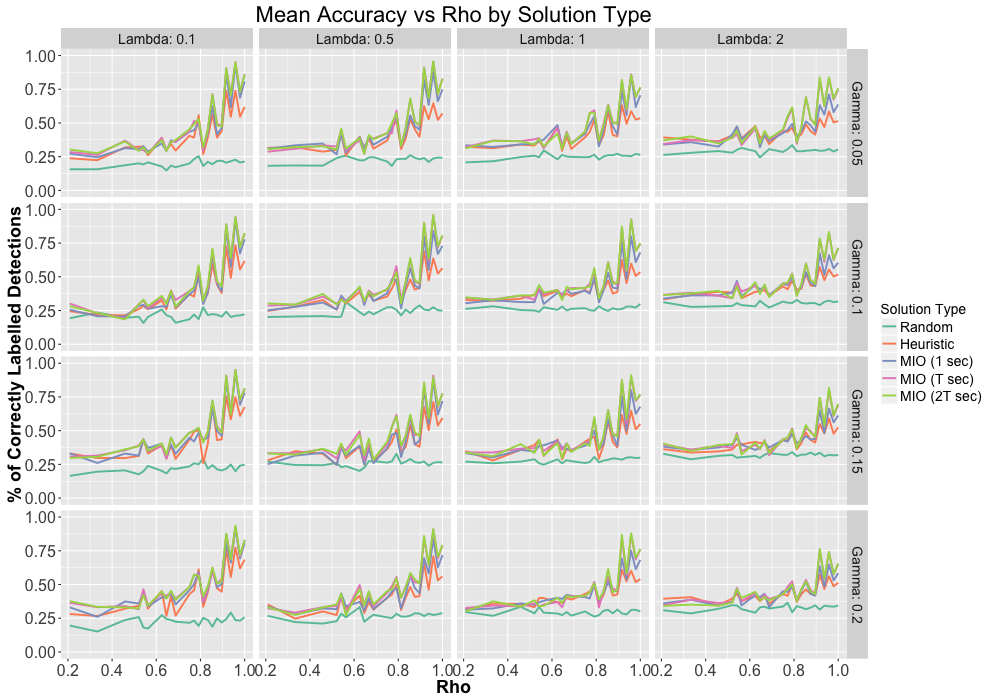
\includegraphics[width=\columnwidth]{../Figures/4_8_Accuracy}
  \caption{Accuracy of robust heuristic and MIO as compared to random solutions for scenarios of 4 targets and 8 scans, arranged by $\gamma$ and $\lambda$.}
  \label{fig:Robust_4_8_Accuracy}
\end{figure}

\begin{figure}[ht]
  \centering
  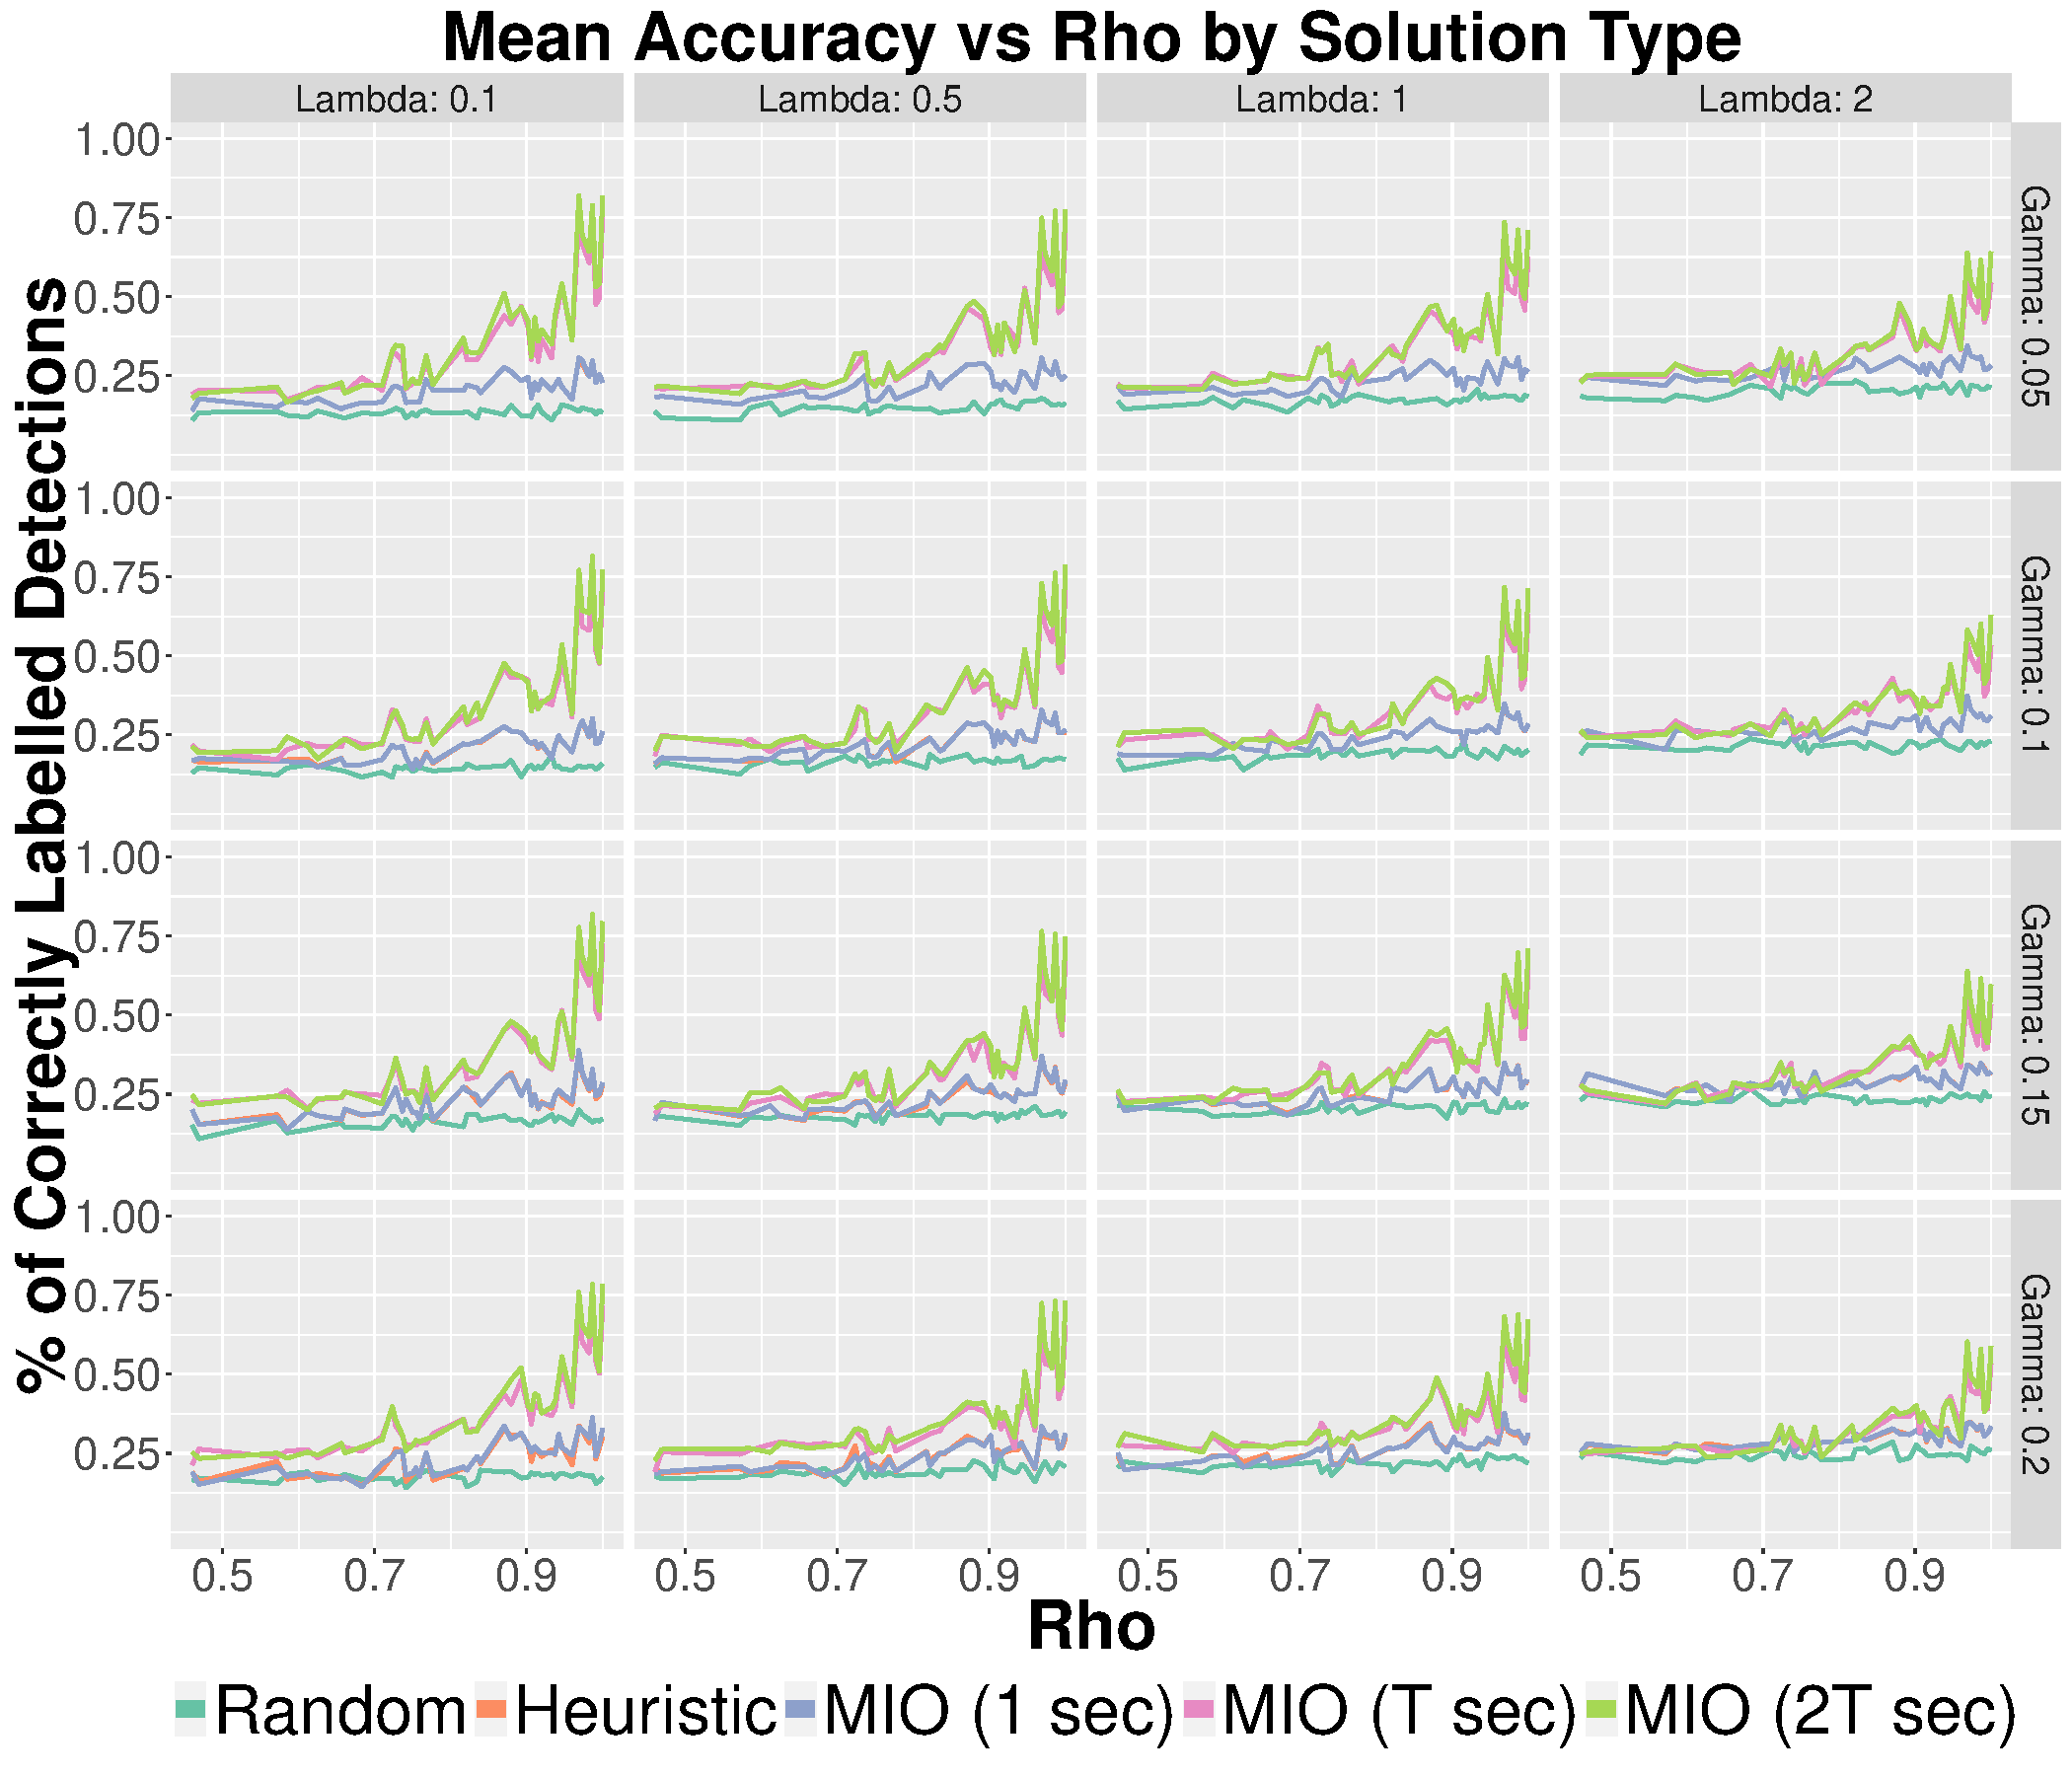
\includegraphics[width=\columnwidth]{../Figures/8_8_Accuracy}
  \caption{Accuracy of robust heuristic and MIO as compared to random solutions for scenarios of 8 targets and 8 scans, arranged by $\gamma$ and $\lambda$.}
  \label{fig:Robust_8_8_Accuracy}
\end{figure}

Similar to the performance of the basic heuristic, we again see that the robust heuristic improves greatly over that of a random solution, and the MIO offers even further improvement. Again, we seeing that running the MIO for 1 second offers significant improvements over the heuristic, and running the MIO for T seconds offers further improvement. However, running the MIO for 2T seconds offers little to no further improvement. Again, these results support the use of the MIO in an online algorithm with a sliding window as mentioned previously. 

Comparing Figure~\ref{fig:Robust_4_8_Accuracy} with the 4 target and 8 scan element of Figure~\ref{fig:Basic_Accuracy_Summary}, we see only a slight decrease in performance when $\gamma = 0.05$ and $\lambda=0.1$. This is an important result because we no longer know the number of targets in the robust case, yet we achieve almost the same levels of accuracy. Furthermore, both Figure~\ref{fig:Robust_4_8_Accuracy} and Figure~\ref{fig:Robust_8_8_Accuracy} show that the robust algorithms are more robust to decreases in the detection probability $\gamma$ than to increases in the false alarm rate $\lambda$. We conclude that the robust approaches are more sensitive to changes in the false alarm rate, in particular when it comes to making data associations. 

We have shown that both the heuristic and the MIO tend to underestimate the number of targets, due to the chosen penalties. We have also shown that accuracy degrades as the false alarm rate increases. This is likely not a coincidence. It is probable that as a result of underestimation, in which fewer trajectories are generated, there is a higher rate of misclassification of detections as false alarms, which in turn directly leads to a reduced accuracy. Therefore, it is a promising result to see accuracies above 75\% in Figure~\ref{fig:Robust_8_8_Accuracy}, even when Figure~\ref{fig:Robust_8_8_Histogram} suggests overestimation. It is entirely possible that further parameter tuning or introducing more complex penalties would lead to even great performance in the data association problem.

\mysubsubsection{Trajectory Estimation}
We conclude our analysis of the robust approaches with a discussion on their performance in the sphere of the trajectory estimation problem. Figures~\ref{fig:Robust_4_8_Delta} and~\ref{fig:Robust_8_8_Delta} plot the $\delta$ performance metric against the difficulty metric, $\sigma$, for scenarios of four and eight targets, respectively. Again, both scenarios have eight scans and both Figures have been arranged by $\gamma$ and $\lambda$. Note that the range on $\sigma$ has been reduced from $[0.1,5.0]$ to $[0.1, 2.0]$. 

\begin{figure}[ht]
  \centering
  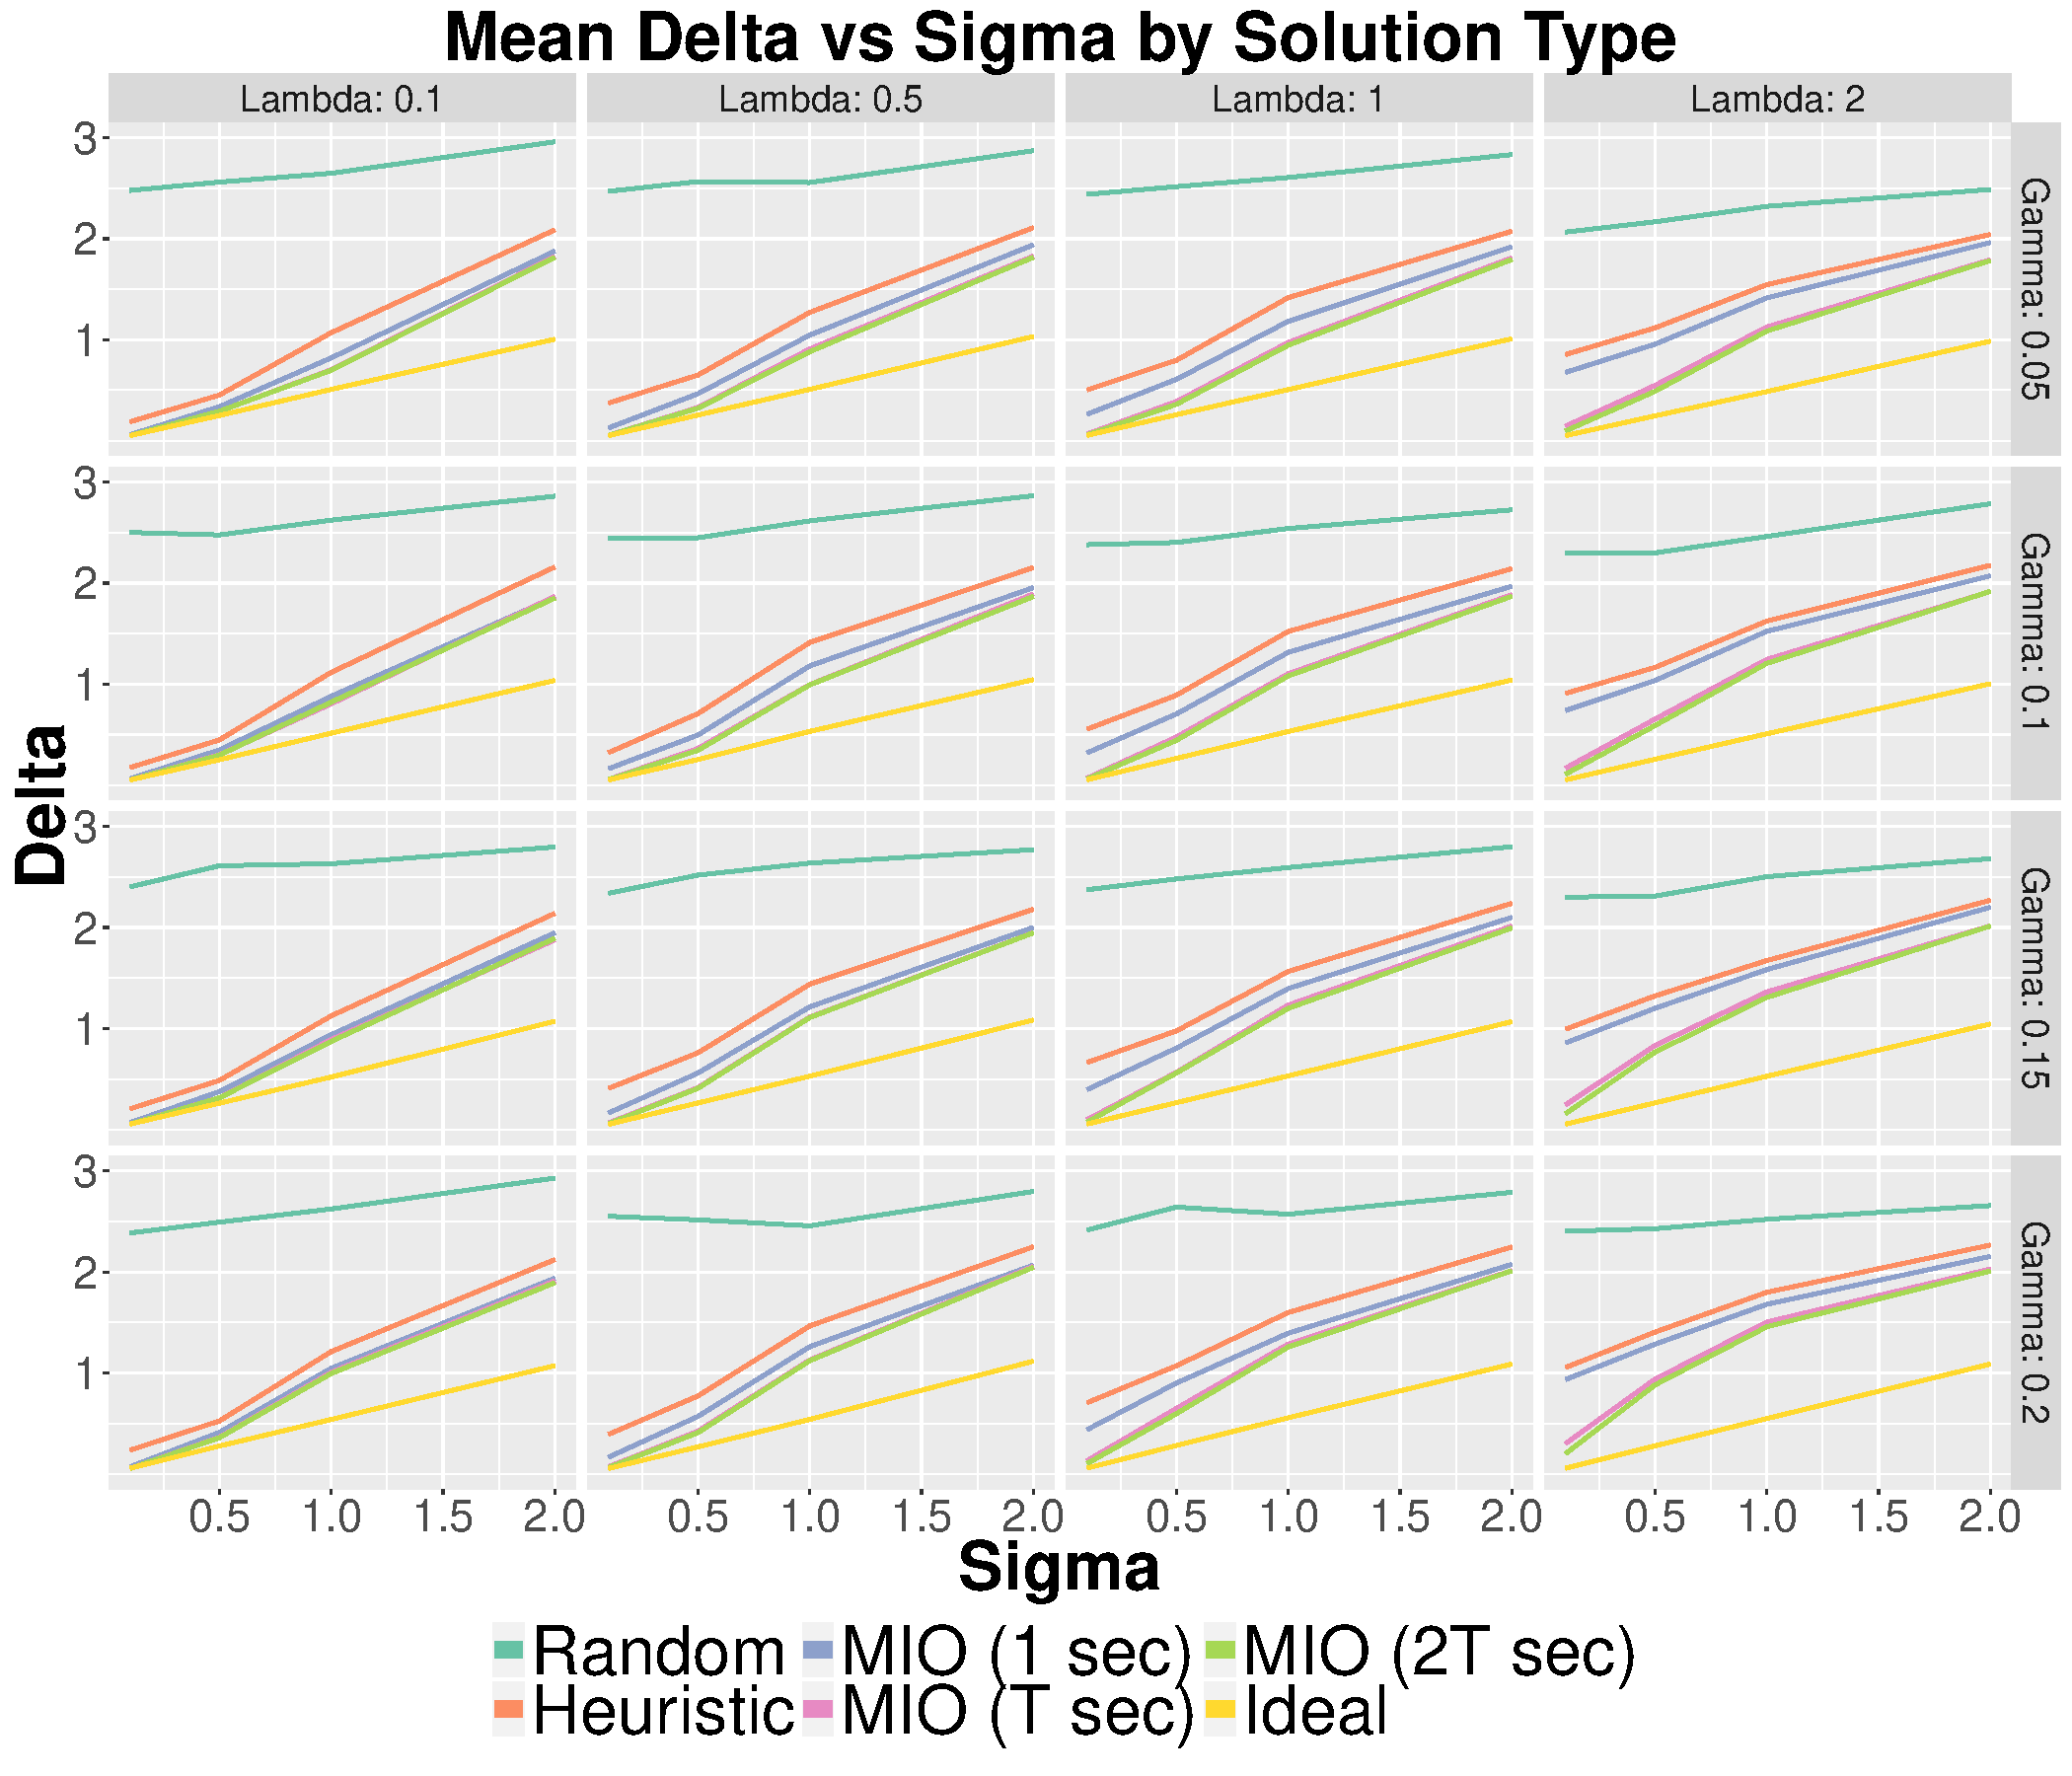
\includegraphics[width=\columnwidth]{../Figures/4_8_Delta}
  \caption{$\delta$ of robust heuristic and MIO as compared to random solutions for scenarios of 4 targets and 8 scans.}
  \label{fig:Robust_4_8_Delta}
\end{figure}

\begin{figure}[ht]
  \centering
  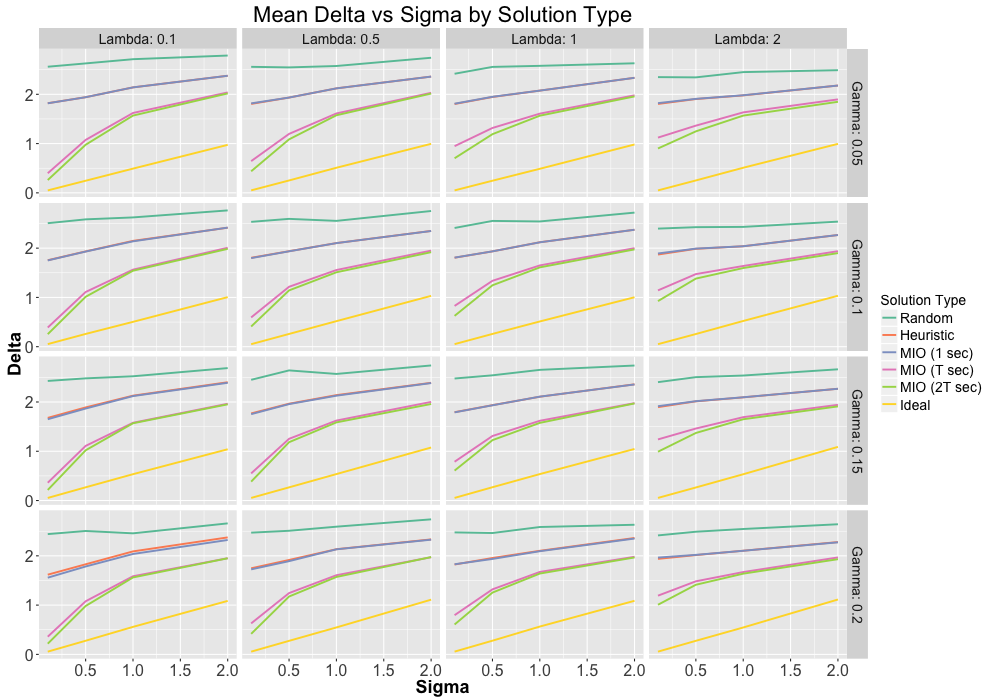
\includegraphics[width=\columnwidth]{../Figures/8_8_Delta}
  \caption{$\delta$ of robust heuristic and MIO as compared to random solutions for scenarios of 8 targets and 8 scans.}
  \label{fig:Robust_8_8_Delta}
\end{figure}

Again, we measure against the basic approaches by comparing Figure~\ref{fig:Robust_4_8_Delta} with the 4 target and 8 scan element of Figure~\ref{Fig:Basic_Delta_Summary}. We see that the robust approaches do not drastically reduce in performance for the easiest robust scenario of $\gamma = 0.05$ and $\lambda = 0.1$. However, the gap in performance between the ideal solution and the solutions of the robust algorithms grows wider with increases in $\sigma$, something that is expected but was not as sizable in the basic experiment. Therefore, the robust approaches may be less robust to increases in $\sigma$ in scenarios with detection ambiguity. However, it also appears that these methods are more robust to increases in the false alarm rate $\lambda$ when it comes to trajectory estimation than they were when it came to data association, especially in the larger scenario shown in Figure~\ref{fig:Robust_8_8_Delta}. We conclude that our robust methods are fairly robust to both increases in the false alarm rate and decreases in trajectory estimation under detection ambiguity, but increasing the signal noise degrades the performance of our methods more so in scenarios with detection ambiguity than in scenarios without detection ambiguity.

In summary,.....discussion on robust summary


